% Options for packages loaded elsewhere
\PassOptionsToPackage{unicode}{hyperref}
\PassOptionsToPackage{hyphens}{url}
%
\documentclass[
]{book}
\usepackage{amsmath,amssymb}
\usepackage{iftex}
\ifPDFTeX
  \usepackage[T1]{fontenc}
  \usepackage[utf8]{inputenc}
  \usepackage{textcomp} % provide euro and other symbols
\else % if luatex or xetex
  \usepackage{unicode-math} % this also loads fontspec
  \defaultfontfeatures{Scale=MatchLowercase}
  \defaultfontfeatures[\rmfamily]{Ligatures=TeX,Scale=1}
\fi
\usepackage{lmodern}
\ifPDFTeX\else
  % xetex/luatex font selection
\fi
% Use upquote if available, for straight quotes in verbatim environments
\IfFileExists{upquote.sty}{\usepackage{upquote}}{}
\IfFileExists{microtype.sty}{% use microtype if available
  \usepackage[]{microtype}
  \UseMicrotypeSet[protrusion]{basicmath} % disable protrusion for tt fonts
}{}
\makeatletter
\@ifundefined{KOMAClassName}{% if non-KOMA class
  \IfFileExists{parskip.sty}{%
    \usepackage{parskip}
  }{% else
    \setlength{\parindent}{0pt}
    \setlength{\parskip}{6pt plus 2pt minus 1pt}}
}{% if KOMA class
  \KOMAoptions{parskip=half}}
\makeatother
\usepackage{xcolor}
\usepackage{color}
\usepackage{fancyvrb}
\newcommand{\VerbBar}{|}
\newcommand{\VERB}{\Verb[commandchars=\\\{\}]}
\DefineVerbatimEnvironment{Highlighting}{Verbatim}{commandchars=\\\{\}}
% Add ',fontsize=\small' for more characters per line
\usepackage{framed}
\definecolor{shadecolor}{RGB}{248,248,248}
\newenvironment{Shaded}{\begin{snugshade}}{\end{snugshade}}
\newcommand{\AlertTok}[1]{\textcolor[rgb]{0.94,0.16,0.16}{#1}}
\newcommand{\AnnotationTok}[1]{\textcolor[rgb]{0.56,0.35,0.01}{\textbf{\textit{#1}}}}
\newcommand{\AttributeTok}[1]{\textcolor[rgb]{0.13,0.29,0.53}{#1}}
\newcommand{\BaseNTok}[1]{\textcolor[rgb]{0.00,0.00,0.81}{#1}}
\newcommand{\BuiltInTok}[1]{#1}
\newcommand{\CharTok}[1]{\textcolor[rgb]{0.31,0.60,0.02}{#1}}
\newcommand{\CommentTok}[1]{\textcolor[rgb]{0.56,0.35,0.01}{\textit{#1}}}
\newcommand{\CommentVarTok}[1]{\textcolor[rgb]{0.56,0.35,0.01}{\textbf{\textit{#1}}}}
\newcommand{\ConstantTok}[1]{\textcolor[rgb]{0.56,0.35,0.01}{#1}}
\newcommand{\ControlFlowTok}[1]{\textcolor[rgb]{0.13,0.29,0.53}{\textbf{#1}}}
\newcommand{\DataTypeTok}[1]{\textcolor[rgb]{0.13,0.29,0.53}{#1}}
\newcommand{\DecValTok}[1]{\textcolor[rgb]{0.00,0.00,0.81}{#1}}
\newcommand{\DocumentationTok}[1]{\textcolor[rgb]{0.56,0.35,0.01}{\textbf{\textit{#1}}}}
\newcommand{\ErrorTok}[1]{\textcolor[rgb]{0.64,0.00,0.00}{\textbf{#1}}}
\newcommand{\ExtensionTok}[1]{#1}
\newcommand{\FloatTok}[1]{\textcolor[rgb]{0.00,0.00,0.81}{#1}}
\newcommand{\FunctionTok}[1]{\textcolor[rgb]{0.13,0.29,0.53}{\textbf{#1}}}
\newcommand{\ImportTok}[1]{#1}
\newcommand{\InformationTok}[1]{\textcolor[rgb]{0.56,0.35,0.01}{\textbf{\textit{#1}}}}
\newcommand{\KeywordTok}[1]{\textcolor[rgb]{0.13,0.29,0.53}{\textbf{#1}}}
\newcommand{\NormalTok}[1]{#1}
\newcommand{\OperatorTok}[1]{\textcolor[rgb]{0.81,0.36,0.00}{\textbf{#1}}}
\newcommand{\OtherTok}[1]{\textcolor[rgb]{0.56,0.35,0.01}{#1}}
\newcommand{\PreprocessorTok}[1]{\textcolor[rgb]{0.56,0.35,0.01}{\textit{#1}}}
\newcommand{\RegionMarkerTok}[1]{#1}
\newcommand{\SpecialCharTok}[1]{\textcolor[rgb]{0.81,0.36,0.00}{\textbf{#1}}}
\newcommand{\SpecialStringTok}[1]{\textcolor[rgb]{0.31,0.60,0.02}{#1}}
\newcommand{\StringTok}[1]{\textcolor[rgb]{0.31,0.60,0.02}{#1}}
\newcommand{\VariableTok}[1]{\textcolor[rgb]{0.00,0.00,0.00}{#1}}
\newcommand{\VerbatimStringTok}[1]{\textcolor[rgb]{0.31,0.60,0.02}{#1}}
\newcommand{\WarningTok}[1]{\textcolor[rgb]{0.56,0.35,0.01}{\textbf{\textit{#1}}}}
\usepackage{longtable,booktabs,array}
\usepackage{calc} % for calculating minipage widths
% Correct order of tables after \paragraph or \subparagraph
\usepackage{etoolbox}
\makeatletter
\patchcmd\longtable{\par}{\if@noskipsec\mbox{}\fi\par}{}{}
\makeatother
% Allow footnotes in longtable head/foot
\IfFileExists{footnotehyper.sty}{\usepackage{footnotehyper}}{\usepackage{footnote}}
\makesavenoteenv{longtable}
\usepackage{graphicx}
\makeatletter
\def\maxwidth{\ifdim\Gin@nat@width>\linewidth\linewidth\else\Gin@nat@width\fi}
\def\maxheight{\ifdim\Gin@nat@height>\textheight\textheight\else\Gin@nat@height\fi}
\makeatother
% Scale images if necessary, so that they will not overflow the page
% margins by default, and it is still possible to overwrite the defaults
% using explicit options in \includegraphics[width, height, ...]{}
\setkeys{Gin}{width=\maxwidth,height=\maxheight,keepaspectratio}
% Set default figure placement to htbp
\makeatletter
\def\fps@figure{htbp}
\makeatother
\setlength{\emergencystretch}{3em} % prevent overfull lines
\providecommand{\tightlist}{%
  \setlength{\itemsep}{0pt}\setlength{\parskip}{0pt}}
\setcounter{secnumdepth}{5}
\usepackage{amsmath}
\usepackage{booktabs}
\usepackage{longtable}
\usepackage{graphicx}
\usepackage{lscape}
\usepackage{array}
\usepackage{caption}
\usepackage{graphicx}
\usepackage{siunitx}
\usepackage[normalem]{ulem}
\usepackage{colortbl}
\usepackage{multirow}
\usepackage{hhline}
\usepackage{calc}
\usepackage{tabularx}
\usepackage{threeparttable}
\usepackage{wrapfig}
\usepackage{adjustbox}
\usepackage{hyperref}
\usepackage{float}
\usepackage{tabularray}
\usepackage[normalem]{ulem}
\usepackage{graphicx}
\usepackage{rotating}
\UseTblrLibrary{booktabs}
\UseTblrLibrary{siunitx}
\NewTableCommand{\tinytableDefineColor}[3]{\definecolor{#1}{#2}{#3}}
\newcommand{\tinytableTabularrayUnderline}[1]{\underline{#1}}
\newcommand{\tinytableTabularrayStrikeout}[1]{\sout{#1}}
\ifLuaTeX
  \usepackage{selnolig}  % disable illegal ligatures
\fi
\usepackage[]{natbib}
\bibliographystyle{plainnat}
\usepackage{bookmark}
\IfFileExists{xurl.sty}{\usepackage{xurl}}{} % add URL line breaks if available
\urlstyle{same}
\hypersetup{
  pdftitle={Terminally Online: Does Donald Trump impact Financial Markets},
  pdfauthor={Marcos Constantinou, Ryan Fellarhi \& Jonas Bruno},
  hidelinks,
  pdfcreator={LaTeX via pandoc}}

\title{Terminally Online: Does Donald Trump impact Financial Markets}
\author{Marcos Constantinou, Ryan Fellarhi \& Jonas Bruno}
\date{Last edited: 12.05.2025}

\begin{document}
\maketitle

{
\setcounter{tocdepth}{1}
\tableofcontents
}
\chapter*{Readme}\label{readme}
\addcontentsline{toc}{chapter}{Readme}

This is a Website for a class project from the 2025 Class Macroeconometrics at Université de Lausanne.

IMPORTANT:use: bookdown::render\_book(``final/index.Rmd'') to render site

\section*{Usage}\label{usage}
\addcontentsline{toc}{section}{Usage}

You can find all sections on the left. There is the Main Report which we hand in. This serves as a complete collection of the whole project to make sure everything is available to readers.

\chapter*{Abstract}\label{abstract}
\addcontentsline{toc}{chapter}{Abstract}

This Project assesses to what extent Financial Markets react to information provided by Donald Trump on Twitter and Truth Social. We asses the impact of posts on hourly volatility using ARMA-X. We evaluate multiple time horizons and independent variables, such as if Trump posts anything, specific words such as tariff and sentiments. We then calculate IRFs and show that there are significant impacts on volatility.

\chapter{Introduction}\label{introduction}

Over the past 15 years social media has become an important
communication tool for politicians. One of the pioneers of this novel
approach has been Donald Trump, the 45th and 47th President of the United
States. Since his ban on Twitter after the January 6th riots, his quantity of
social media posts has drastically increased. This is shown in the following
figure. \footnote{Includes both Posts and Reposts}

The content of his posts can sometimes have announcements or teases of future
political decisions. Note the recent infamous ``THIS IS A GREAT TIME TO BUY!!! DJT''
post sent just an hour before lifting his reciprocal tariffs. It is then not
improbable that agents in financial markets might take this information into
account in their decision making. This question has been asked before in the
literature, focusing rather on his first term.

This brings us to our research question: Do Donald Trumps Posts impact market Volatility?

\ref{fig:fig1}

\begin{figure}
\centering
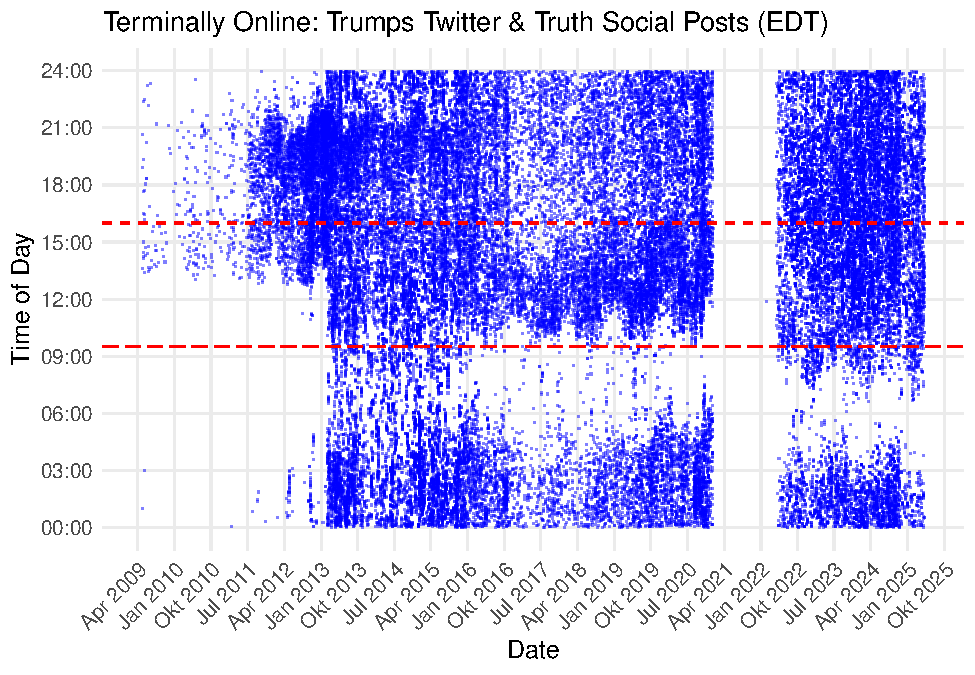
\includegraphics{_main_files/figure-latex/fig1-1.pdf}
\caption{\label{fig:fig1}Terminally Online: Trump's Twitter \& Truth Social Posts (EDT)}
\end{figure}

\section{Literature Review}\label{literature-review}

Information is one of the most valuable assets in the financial market.
Its importance lies at the core of the ``Efficient Market Hypothesis'',
which states that the prices of assets fully reflect all
available information, adjusting immediately to any new data
\citet{famaAdjustmentStockPrices2003} , and thereby creating a strong demand
for information flow. In addition, the ``Mixture of Distribution
Hypothesis'' states that the release of new information is closely linked
to movements in both realized and implied volatility (1)(3)(7).

Consequently, a large part of the literature had focused on the relation
between announcements, news and market activity. For example,
\citet{schumakerTextualAnalysisStock2009} use various linguistic and textual
representations derived from financial news to predict stock market
prices. Similarly, \citet{ederingtonHowMarketsProcess1993} analyze the impact
of macroeconomic news announcements on interest rate and foreign
exchange futures markets, particularly in terms of price changes and
volatility. Both studies, among others, find that prices--- such as stock
prices---react primarily within minutes after the release of new
information.

Recently, the world has witnessed the rise of the Internet
which revolutionized the dissemination and accessibility of information.
Social media enable investors, analysts or politicians to instantly
share their information, news or opinions. This led some studies to
focus on the communication dynamics of social platform to predict
changes in the returns of financial assets (6)(8). In this context, the
impact of Trump's tweets on various financial and macroeconomic
variables has been analysed by several studies, especially during his
first mandate.

Using high-frequency financial data,
\citet{gjerstadPresidentTrumpsTweets2021} found an increase in uncertainty and
trading volume, along with a decline in the U.S. stock market---regardless
of the tweet's content. However, the effect was stronger when Trump used
confrontational words such as ``tariff'' or ``trade war.'' Some of his
announcements also influenced the U.S. dollar exchange rate (l) and
certain market indices within minutes of the tweet being posted (r)(a).

Other scholars have shown that negative Trump tweets about specific
companies tended to reduce demand for their stocks (b)(g), whereas some
other have shown that they also impact market volatility indices such as
the VIX (w) or the Volfele(v). The effects of his tweets also extended
beyond the U.S.. For example, \citet{nishimuraImpactsDonaldTrumps2025} shows a
positive relationship between volatility in European stock markets and
tweeter activity of Trump, and this effect tends to intensify as public
intention for his tweet grows (z).

Our paper is built as follows:

\chapter{Data}\label{data}

\section{Financial Data}\label{financial-data}

For our financial data, we decided to try to find minute-by-minute prices for
broad market indices. While the actual indices do not update their prices so often,
we had to take proxies under the form of ETF's that track them. Our 3 markets of
analysis are: SPY to track the S\&P500, VGK to track the FTSE Developed Europe
All Cap Index, and finally ASHR to track the CSI 300 China. We accessed this data
through a free stock API, Alpha Vantage. Our timeframe is from the first
of January 2014 to the 7th of May 2025.

We then had to transform this data to get our main variable of interest, Average
Hourly Volatility (AHV). Note that this is realised market volatility. We did so
with the following formula:
\[
\begin{aligned}
  v_t = \frac{1}{N}&\sum_{i=1}^N(\Delta p_{t,i})^2 
\end{aligned}
\]
Where \(\Delta p_t\) is the difference in price (open - close) and \(i\) represents
every minute.

We used a custom function in order to get the AHV for each open market hour. Note
that the first hour is from 9:30 am to 10:00 am since the
market open on a half-hour but closes at 4:00 pm. We can plot this data in
{ \emph{figX} }.

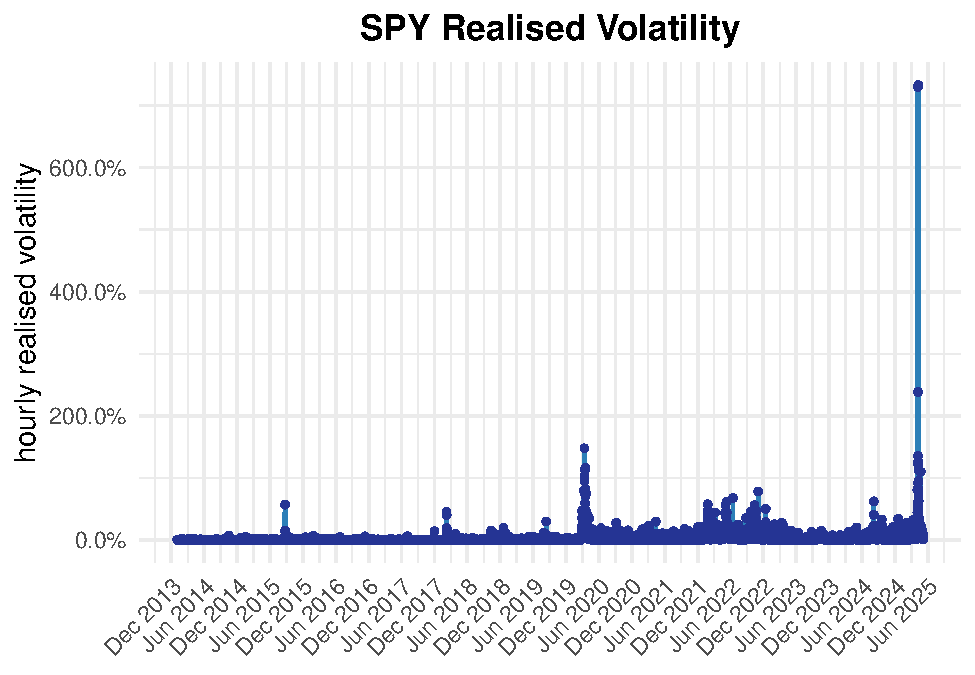
\includegraphics{_main_files/figure-latex/fin plots-1.pdf} 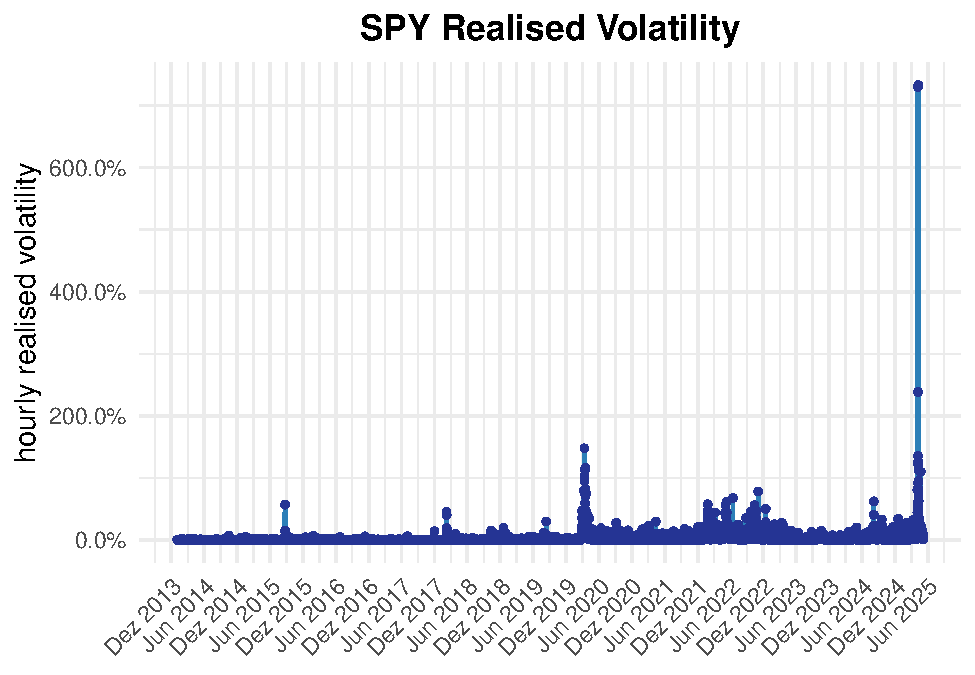
\includegraphics{_main_files/figure-latex/fin plots-2.pdf}

\section{Political Data}\label{political-data}

We have two sources for Trump's posts. The Tweets are from Kaggle
\citet{DonaldTrumpTweets} and go until the 8th of January 2021. Since he
switched his primary Posting platform to Truth Social we use only that
Data from 2021 onwards. All Truth Social Posts were scrapped from
trumpstruth.org, a webpage that aims to conserve all his posts. You can
find the dataset, and webscrapper, and Data cleaning process in the
Appendix.

Since we're using financial data that is constrained by trading hours,
we decided to move posts after 16:00 to the next trading day's opening
hour.

A big problem we had in our analysis was what to do with social media posts
which appeared outside market hours. We first decided to simply ignore them, but
it turned out to remove a lot of observations. We finally decided to push all the
social media information outside market hours to the next open hour. This comes
as an assumption.\footnote{2}

Since our financial data is hourly, we aggregate the social data by hour. We
then construct multiple variables from the social media data. These include
a dummy for whether there was a post, the number of posts an hour and counts
for certain words (``tariffs'',``trade'',``china''). Further we applied some simple
sentiment analysis algorithms on the data to see if there are certain sentiments
in his tweets that move the markets. More information and detailed process are in
the appendix and online.

{ \emph{insert wordcloud} }.

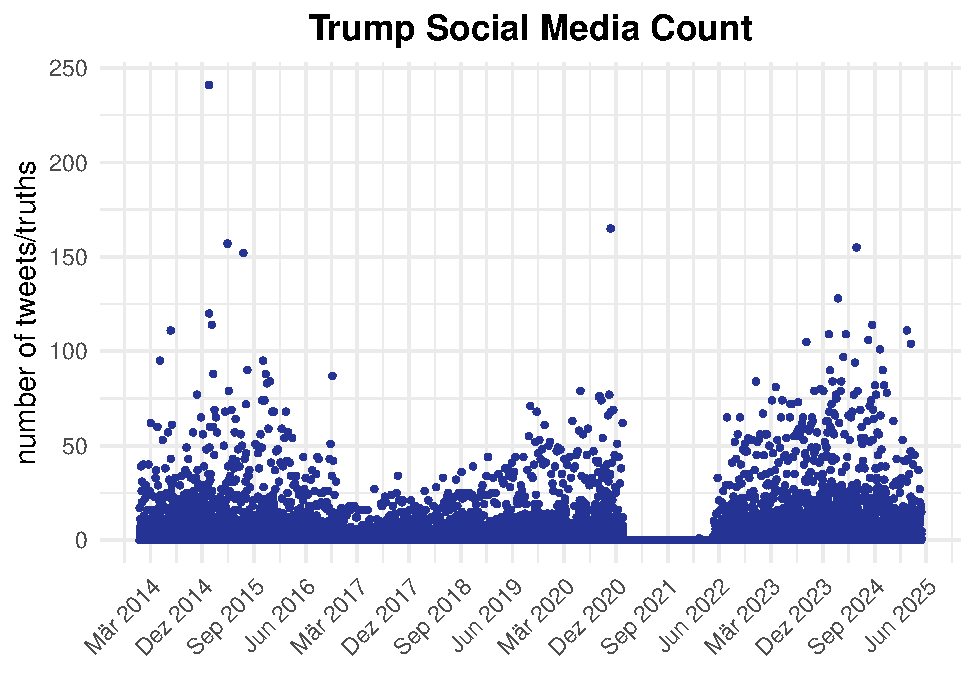
\includegraphics{_main_files/figure-latex/social plots-1.pdf}

\section{Final Dataframe}\label{final-dataframe}

 
  \providecommand{\huxb}[2]{\arrayrulecolor[RGB]{#1}\global\arrayrulewidth=#2pt}
  \providecommand{\huxvb}[2]{\color[RGB]{#1}\vrule width #2pt}
  \providecommand{\huxtpad}[1]{\rule{0pt}{#1}}
  \providecommand{\huxbpad}[1]{\rule[-#1]{0pt}{#1}}

\begin{table}[ht]
\begin{centerbox}
\begin{threeparttable}
\captionsetup{justification=centering,singlelinecheck=off}
\caption{\label{tab:data} }
 \setlength{\tabcolsep}{0pt}
\begin{tabular}{l l l l}


\hhline{>{\huxb{0, 0, 0}{0.4}}->{\huxb{0, 0, 0}{0.4}}->{\huxb{0, 0, 0}{0.4}}->{\huxb{0, 0, 0}{0.4}}-}
\arrayrulecolor{black}

\multicolumn{1}{!{\huxvb{0, 0, 0}{0.4}}r!{\huxvb{0, 0, 0}{0}}}{\huxtpad{6pt + 1em}\raggedleft \hspace{6pt} \textbf{timestamp} \hspace{6pt}\huxbpad{6pt}} &
\multicolumn{1}{r!{\huxvb{0, 0, 0}{0}}}{\huxtpad{6pt + 1em}\raggedleft \hspace{6pt} \textbf{SPY\_vol} \hspace{6pt}\huxbpad{6pt}} &
\multicolumn{1}{r!{\huxvb{0, 0, 0}{0}}}{\huxtpad{6pt + 1em}\raggedleft \hspace{6pt} \textbf{VGK\_vol} \hspace{6pt}\huxbpad{6pt}} &
\multicolumn{1}{r!{\huxvb{0, 0, 0}{0.4}}}{\huxtpad{6pt + 1em}\raggedleft \hspace{6pt} \textbf{ASHR\_vol} \hspace{6pt}\huxbpad{6pt}} \tabularnewline[-0.5pt]


\hhline{>{\huxb{0, 0, 0}{0.4}}->{\huxb{0, 0, 0}{0.4}}->{\huxb{0, 0, 0}{0.4}}->{\huxb{0, 0, 0}{0.4}}-}
\arrayrulecolor{black}

\multicolumn{1}{!{\huxvb{0, 0, 0}{0.4}}r!{\huxvb{0, 0, 0}{0}}}{\cellcolor[RGB]{242, 242, 242}\huxtpad{6pt + 1em}\raggedleft \hspace{6pt} 2025-05-06 10:00:00 \hspace{6pt}\huxbpad{6pt}} &
\multicolumn{1}{r!{\huxvb{0, 0, 0}{0}}}{\cellcolor[RGB]{242, 242, 242}\huxtpad{6pt + 1em}\raggedleft \hspace{6pt} 0.0466 \hspace{6pt}\huxbpad{6pt}} &
\multicolumn{1}{r!{\huxvb{0, 0, 0}{0}}}{\cellcolor[RGB]{242, 242, 242}\huxtpad{6pt + 1em}\raggedleft \hspace{6pt} 0.000731 \hspace{6pt}\huxbpad{6pt}} &
\multicolumn{1}{r!{\huxvb{0, 0, 0}{0.4}}}{\cellcolor[RGB]{242, 242, 242}\huxtpad{6pt + 1em}\raggedleft \hspace{6pt} 5.32e-05 \hspace{6pt}\huxbpad{6pt}} \tabularnewline[-0.5pt]


\hhline{>{\huxb{0, 0, 0}{0.4}}|>{\huxb{0, 0, 0}{0.4}}|}
\arrayrulecolor{black}

\multicolumn{1}{!{\huxvb{0, 0, 0}{0.4}}r!{\huxvb{0, 0, 0}{0}}}{\huxtpad{6pt + 1em}\raggedleft \hspace{6pt} 2025-05-06 11:00:00 \hspace{6pt}\huxbpad{6pt}} &
\multicolumn{1}{r!{\huxvb{0, 0, 0}{0}}}{\huxtpad{6pt + 1em}\raggedleft \hspace{6pt} 0.0278 \hspace{6pt}\huxbpad{6pt}} &
\multicolumn{1}{r!{\huxvb{0, 0, 0}{0}}}{\huxtpad{6pt + 1em}\raggedleft \hspace{6pt} 0.000217 \hspace{6pt}\huxbpad{6pt}} &
\multicolumn{1}{r!{\huxvb{0, 0, 0}{0.4}}}{\huxtpad{6pt + 1em}\raggedleft \hspace{6pt} 3.33e-05 \hspace{6pt}\huxbpad{6pt}} \tabularnewline[-0.5pt]


\hhline{>{\huxb{0, 0, 0}{0.4}}|>{\huxb{0, 0, 0}{0.4}}|}
\arrayrulecolor{black}

\multicolumn{1}{!{\huxvb{0, 0, 0}{0.4}}r!{\huxvb{0, 0, 0}{0}}}{\cellcolor[RGB]{242, 242, 242}\huxtpad{6pt + 1em}\raggedleft \hspace{6pt} 2025-05-06 12:00:00 \hspace{6pt}\huxbpad{6pt}} &
\multicolumn{1}{r!{\huxvb{0, 0, 0}{0}}}{\cellcolor[RGB]{242, 242, 242}\huxtpad{6pt + 1em}\raggedleft \hspace{6pt} 0.0859 \hspace{6pt}\huxbpad{6pt}} &
\multicolumn{1}{r!{\huxvb{0, 0, 0}{0}}}{\cellcolor[RGB]{242, 242, 242}\huxtpad{6pt + 1em}\raggedleft \hspace{6pt} 0.000468 \hspace{6pt}\huxbpad{6pt}} &
\multicolumn{1}{r!{\huxvb{0, 0, 0}{0.4}}}{\cellcolor[RGB]{242, 242, 242}\huxtpad{6pt + 1em}\raggedleft \hspace{6pt} 3e-05\hphantom{0}\hphantom{0}\hphantom{0}\hphantom{0}\hphantom{0}\hphantom{0}\hphantom{0} \hspace{6pt}\huxbpad{6pt}} \tabularnewline[-0.5pt]


\hhline{>{\huxb{0, 0, 0}{0.4}}|>{\huxb{0, 0, 0}{0.4}}|}
\arrayrulecolor{black}

\multicolumn{1}{!{\huxvb{0, 0, 0}{0.4}}r!{\huxvb{0, 0, 0}{0}}}{\huxtpad{6pt + 1em}\raggedleft \hspace{6pt} 2025-05-06 13:00:00 \hspace{6pt}\huxbpad{6pt}} &
\multicolumn{1}{r!{\huxvb{0, 0, 0}{0}}}{\huxtpad{6pt + 1em}\raggedleft \hspace{6pt} 0.0457 \hspace{6pt}\huxbpad{6pt}} &
\multicolumn{1}{r!{\huxvb{0, 0, 0}{0}}}{\huxtpad{6pt + 1em}\raggedleft \hspace{6pt} 0.000457 \hspace{6pt}\huxbpad{6pt}} &
\multicolumn{1}{r!{\huxvb{0, 0, 0}{0.4}}}{\huxtpad{6pt + 1em}\raggedleft \hspace{6pt} 3.26e-05 \hspace{6pt}\huxbpad{6pt}} \tabularnewline[-0.5pt]


\hhline{>{\huxb{0, 0, 0}{0.4}}|>{\huxb{0, 0, 0}{0.4}}|}
\arrayrulecolor{black}

\multicolumn{1}{!{\huxvb{0, 0, 0}{0.4}}r!{\huxvb{0, 0, 0}{0}}}{\cellcolor[RGB]{242, 242, 242}\huxtpad{6pt + 1em}\raggedleft \hspace{6pt} 2025-05-06 14:00:00 \hspace{6pt}\huxbpad{6pt}} &
\multicolumn{1}{r!{\huxvb{0, 0, 0}{0}}}{\cellcolor[RGB]{242, 242, 242}\huxtpad{6pt + 1em}\raggedleft \hspace{6pt} 0.0336 \hspace{6pt}\huxbpad{6pt}} &
\multicolumn{1}{r!{\huxvb{0, 0, 0}{0}}}{\cellcolor[RGB]{242, 242, 242}\huxtpad{6pt + 1em}\raggedleft \hspace{6pt} 0.000224 \hspace{6pt}\huxbpad{6pt}} &
\multicolumn{1}{r!{\huxvb{0, 0, 0}{0.4}}}{\cellcolor[RGB]{242, 242, 242}\huxtpad{6pt + 1em}\raggedleft \hspace{6pt} 2.24e-05 \hspace{6pt}\huxbpad{6pt}} \tabularnewline[-0.5pt]


\hhline{>{\huxb{0, 0, 0}{0.4}}|>{\huxb{0, 0, 0}{0.4}}|}
\arrayrulecolor{black}

\multicolumn{1}{!{\huxvb{0, 0, 0}{0.4}}r!{\huxvb{0, 0, 0}{0}}}{\huxtpad{6pt + 1em}\raggedleft \hspace{6pt} 2025-05-06 15:00:00 \hspace{6pt}\huxbpad{6pt}} &
\multicolumn{1}{r!{\huxvb{0, 0, 0}{0}}}{\huxtpad{6pt + 1em}\raggedleft \hspace{6pt} 0.0517 \hspace{6pt}\huxbpad{6pt}} &
\multicolumn{1}{r!{\huxvb{0, 0, 0}{0}}}{\huxtpad{6pt + 1em}\raggedleft \hspace{6pt} 0.000295 \hspace{6pt}\huxbpad{6pt}} &
\multicolumn{1}{r!{\huxvb{0, 0, 0}{0.4}}}{\huxtpad{6pt + 1em}\raggedleft \hspace{6pt} 2.03e-05 \hspace{6pt}\huxbpad{6pt}} \tabularnewline[-0.5pt]


\hhline{>{\huxb{0, 0, 0}{0.4}}->{\huxb{0, 0, 0}{0.4}}->{\huxb{0, 0, 0}{0.4}}->{\huxb{0, 0, 0}{0.4}}-}
\arrayrulecolor{black}
\end{tabular}
\end{threeparttable}\par\end{centerbox}

\end{table}
 

 
  \providecommand{\huxb}[2]{\arrayrulecolor[RGB]{#1}\global\arrayrulewidth=#2pt}
  \providecommand{\huxvb}[2]{\color[RGB]{#1}\vrule width #2pt}
  \providecommand{\huxtpad}[1]{\rule{0pt}{#1}}
  \providecommand{\huxbpad}[1]{\rule[-#1]{0pt}{#1}}

\begin{table}[ht]
\begin{centerbox}
\begin{threeparttable}
\captionsetup{justification=centering,singlelinecheck=off}
\caption{\label{tab:data} }
 \setlength{\tabcolsep}{0pt}
\begin{tabular}{l l l l l}


\hhline{>{\huxb{0, 0, 0}{0.4}}->{\huxb{0, 0, 0}{0.4}}->{\huxb{0, 0, 0}{0.4}}->{\huxb{0, 0, 0}{0.4}}->{\huxb{0, 0, 0}{0.4}}-}
\arrayrulecolor{black}

\multicolumn{1}{!{\huxvb{0, 0, 0}{0.4}}r!{\huxvb{0, 0, 0}{0}}}{\huxtpad{6pt + 1em}\raggedleft \hspace{6pt} \textbf{dummy} \hspace{6pt}\huxbpad{6pt}} &
\multicolumn{1}{r!{\huxvb{0, 0, 0}{0}}}{\huxtpad{6pt + 1em}\raggedleft \hspace{6pt} \textbf{N} \hspace{6pt}\huxbpad{6pt}} &
\multicolumn{1}{r!{\huxvb{0, 0, 0}{0}}}{\huxtpad{6pt + 1em}\raggedleft \hspace{6pt} \textbf{tariff} \hspace{6pt}\huxbpad{6pt}} &
\multicolumn{1}{r!{\huxvb{0, 0, 0}{0}}}{\huxtpad{6pt + 1em}\raggedleft \hspace{6pt} \textbf{trade} \hspace{6pt}\huxbpad{6pt}} &
\multicolumn{1}{r!{\huxvb{0, 0, 0}{0.4}}}{\huxtpad{6pt + 1em}\raggedleft \hspace{6pt} \textbf{china} \hspace{6pt}\huxbpad{6pt}} \tabularnewline[-0.5pt]


\hhline{>{\huxb{0, 0, 0}{0.4}}->{\huxb{0, 0, 0}{0.4}}->{\huxb{0, 0, 0}{0.4}}->{\huxb{0, 0, 0}{0.4}}->{\huxb{0, 0, 0}{0.4}}-}
\arrayrulecolor{black}

\multicolumn{1}{!{\huxvb{0, 0, 0}{0.4}}r!{\huxvb{0, 0, 0}{0}}}{\cellcolor[RGB]{242, 242, 242}\huxtpad{6pt + 1em}\raggedleft \hspace{6pt} 0 \hspace{6pt}\huxbpad{6pt}} &
\multicolumn{1}{r!{\huxvb{0, 0, 0}{0}}}{\cellcolor[RGB]{242, 242, 242}\huxtpad{6pt + 1em}\raggedleft \hspace{6pt} 0 \hspace{6pt}\huxbpad{6pt}} &
\multicolumn{1}{r!{\huxvb{0, 0, 0}{0}}}{\cellcolor[RGB]{242, 242, 242}\huxtpad{6pt + 1em}\raggedleft \hspace{6pt} 0 \hspace{6pt}\huxbpad{6pt}} &
\multicolumn{1}{r!{\huxvb{0, 0, 0}{0}}}{\cellcolor[RGB]{242, 242, 242}\huxtpad{6pt + 1em}\raggedleft \hspace{6pt} 0 \hspace{6pt}\huxbpad{6pt}} &
\multicolumn{1}{r!{\huxvb{0, 0, 0}{0.4}}}{\cellcolor[RGB]{242, 242, 242}\huxtpad{6pt + 1em}\raggedleft \hspace{6pt} 0 \hspace{6pt}\huxbpad{6pt}} \tabularnewline[-0.5pt]


\hhline{>{\huxb{0, 0, 0}{0.4}}|>{\huxb{0, 0, 0}{0.4}}|}
\arrayrulecolor{black}

\multicolumn{1}{!{\huxvb{0, 0, 0}{0.4}}r!{\huxvb{0, 0, 0}{0}}}{\huxtpad{6pt + 1em}\raggedleft \hspace{6pt} 0 \hspace{6pt}\huxbpad{6pt}} &
\multicolumn{1}{r!{\huxvb{0, 0, 0}{0}}}{\huxtpad{6pt + 1em}\raggedleft \hspace{6pt} 0 \hspace{6pt}\huxbpad{6pt}} &
\multicolumn{1}{r!{\huxvb{0, 0, 0}{0}}}{\huxtpad{6pt + 1em}\raggedleft \hspace{6pt} 0 \hspace{6pt}\huxbpad{6pt}} &
\multicolumn{1}{r!{\huxvb{0, 0, 0}{0}}}{\huxtpad{6pt + 1em}\raggedleft \hspace{6pt} 0 \hspace{6pt}\huxbpad{6pt}} &
\multicolumn{1}{r!{\huxvb{0, 0, 0}{0.4}}}{\huxtpad{6pt + 1em}\raggedleft \hspace{6pt} 0 \hspace{6pt}\huxbpad{6pt}} \tabularnewline[-0.5pt]


\hhline{>{\huxb{0, 0, 0}{0.4}}|>{\huxb{0, 0, 0}{0.4}}|}
\arrayrulecolor{black}

\multicolumn{1}{!{\huxvb{0, 0, 0}{0.4}}r!{\huxvb{0, 0, 0}{0}}}{\cellcolor[RGB]{242, 242, 242}\huxtpad{6pt + 1em}\raggedleft \hspace{6pt} 1 \hspace{6pt}\huxbpad{6pt}} &
\multicolumn{1}{r!{\huxvb{0, 0, 0}{0}}}{\cellcolor[RGB]{242, 242, 242}\huxtpad{6pt + 1em}\raggedleft \hspace{6pt} 3 \hspace{6pt}\huxbpad{6pt}} &
\multicolumn{1}{r!{\huxvb{0, 0, 0}{0}}}{\cellcolor[RGB]{242, 242, 242}\huxtpad{6pt + 1em}\raggedleft \hspace{6pt} 0 \hspace{6pt}\huxbpad{6pt}} &
\multicolumn{1}{r!{\huxvb{0, 0, 0}{0}}}{\cellcolor[RGB]{242, 242, 242}\huxtpad{6pt + 1em}\raggedleft \hspace{6pt} 2 \hspace{6pt}\huxbpad{6pt}} &
\multicolumn{1}{r!{\huxvb{0, 0, 0}{0.4}}}{\cellcolor[RGB]{242, 242, 242}\huxtpad{6pt + 1em}\raggedleft \hspace{6pt} 0 \hspace{6pt}\huxbpad{6pt}} \tabularnewline[-0.5pt]


\hhline{>{\huxb{0, 0, 0}{0.4}}|>{\huxb{0, 0, 0}{0.4}}|}
\arrayrulecolor{black}

\multicolumn{1}{!{\huxvb{0, 0, 0}{0.4}}r!{\huxvb{0, 0, 0}{0}}}{\huxtpad{6pt + 1em}\raggedleft \hspace{6pt} 1 \hspace{6pt}\huxbpad{6pt}} &
\multicolumn{1}{r!{\huxvb{0, 0, 0}{0}}}{\huxtpad{6pt + 1em}\raggedleft \hspace{6pt} 5 \hspace{6pt}\huxbpad{6pt}} &
\multicolumn{1}{r!{\huxvb{0, 0, 0}{0}}}{\huxtpad{6pt + 1em}\raggedleft \hspace{6pt} 0 \hspace{6pt}\huxbpad{6pt}} &
\multicolumn{1}{r!{\huxvb{0, 0, 0}{0}}}{\huxtpad{6pt + 1em}\raggedleft \hspace{6pt} 0 \hspace{6pt}\huxbpad{6pt}} &
\multicolumn{1}{r!{\huxvb{0, 0, 0}{0.4}}}{\huxtpad{6pt + 1em}\raggedleft \hspace{6pt} 0 \hspace{6pt}\huxbpad{6pt}} \tabularnewline[-0.5pt]


\hhline{>{\huxb{0, 0, 0}{0.4}}|>{\huxb{0, 0, 0}{0.4}}|}
\arrayrulecolor{black}

\multicolumn{1}{!{\huxvb{0, 0, 0}{0.4}}r!{\huxvb{0, 0, 0}{0}}}{\cellcolor[RGB]{242, 242, 242}\huxtpad{6pt + 1em}\raggedleft \hspace{6pt} 1 \hspace{6pt}\huxbpad{6pt}} &
\multicolumn{1}{r!{\huxvb{0, 0, 0}{0}}}{\cellcolor[RGB]{242, 242, 242}\huxtpad{6pt + 1em}\raggedleft \hspace{6pt} 1 \hspace{6pt}\huxbpad{6pt}} &
\multicolumn{1}{r!{\huxvb{0, 0, 0}{0}}}{\cellcolor[RGB]{242, 242, 242}\huxtpad{6pt + 1em}\raggedleft \hspace{6pt} 0 \hspace{6pt}\huxbpad{6pt}} &
\multicolumn{1}{r!{\huxvb{0, 0, 0}{0}}}{\cellcolor[RGB]{242, 242, 242}\huxtpad{6pt + 1em}\raggedleft \hspace{6pt} 0 \hspace{6pt}\huxbpad{6pt}} &
\multicolumn{1}{r!{\huxvb{0, 0, 0}{0.4}}}{\cellcolor[RGB]{242, 242, 242}\huxtpad{6pt + 1em}\raggedleft \hspace{6pt} 0 \hspace{6pt}\huxbpad{6pt}} \tabularnewline[-0.5pt]


\hhline{>{\huxb{0, 0, 0}{0.4}}|>{\huxb{0, 0, 0}{0.4}}|}
\arrayrulecolor{black}

\multicolumn{1}{!{\huxvb{0, 0, 0}{0.4}}r!{\huxvb{0, 0, 0}{0}}}{\huxtpad{6pt + 1em}\raggedleft \hspace{6pt} 0 \hspace{6pt}\huxbpad{6pt}} &
\multicolumn{1}{r!{\huxvb{0, 0, 0}{0}}}{\huxtpad{6pt + 1em}\raggedleft \hspace{6pt} 0 \hspace{6pt}\huxbpad{6pt}} &
\multicolumn{1}{r!{\huxvb{0, 0, 0}{0}}}{\huxtpad{6pt + 1em}\raggedleft \hspace{6pt} 0 \hspace{6pt}\huxbpad{6pt}} &
\multicolumn{1}{r!{\huxvb{0, 0, 0}{0}}}{\huxtpad{6pt + 1em}\raggedleft \hspace{6pt} 0 \hspace{6pt}\huxbpad{6pt}} &
\multicolumn{1}{r!{\huxvb{0, 0, 0}{0.4}}}{\huxtpad{6pt + 1em}\raggedleft \hspace{6pt} 0 \hspace{6pt}\huxbpad{6pt}} \tabularnewline[-0.5pt]


\hhline{>{\huxb{0, 0, 0}{0.4}}->{\huxb{0, 0, 0}{0.4}}->{\huxb{0, 0, 0}{0.4}}->{\huxb{0, 0, 0}{0.4}}->{\huxb{0, 0, 0}{0.4}}-}
\arrayrulecolor{black}
\end{tabular}
\end{threeparttable}\par\end{centerbox}

\end{table}
 

 
  \providecommand{\huxb}[2]{\arrayrulecolor[RGB]{#1}\global\arrayrulewidth=#2pt}
  \providecommand{\huxvb}[2]{\color[RGB]{#1}\vrule width #2pt}
  \providecommand{\huxtpad}[1]{\rule{0pt}{#1}}
  \providecommand{\huxbpad}[1]{\rule[-#1]{0pt}{#1}}

\begin{table}[ht]
\begin{centerbox}
\begin{threeparttable}
\captionsetup{justification=centering,singlelinecheck=off}
\caption{\label{tab:data} }
 \setlength{\tabcolsep}{0pt}
\begin{tabular}{l l l l l}


\hhline{>{\huxb{0, 0, 0}{0.4}}->{\huxb{0, 0, 0}{0.4}}->{\huxb{0, 0, 0}{0.4}}->{\huxb{0, 0, 0}{0.4}}->{\huxb{0, 0, 0}{0.4}}-}
\arrayrulecolor{black}

\multicolumn{1}{!{\huxvb{0, 0, 0}{0.4}}r!{\huxvb{0, 0, 0}{0}}}{\huxtpad{6pt + 1em}\raggedleft \hspace{6pt} \textbf{prop\_anger} \hspace{6pt}\huxbpad{6pt}} &
\multicolumn{1}{r!{\huxvb{0, 0, 0}{0}}}{\huxtpad{6pt + 1em}\raggedleft \hspace{6pt} \textbf{prop\_anticipation} \hspace{6pt}\huxbpad{6pt}} &
\multicolumn{1}{r!{\huxvb{0, 0, 0}{0}}}{\huxtpad{6pt + 1em}\raggedleft \hspace{6pt} \textbf{prop\_disgust} \hspace{6pt}\huxbpad{6pt}} &
\multicolumn{1}{r!{\huxvb{0, 0, 0}{0}}}{\huxtpad{6pt + 1em}\raggedleft \hspace{6pt} \textbf{prop\_fear} \hspace{6pt}\huxbpad{6pt}} &
\multicolumn{1}{r!{\huxvb{0, 0, 0}{0.4}}}{\huxtpad{6pt + 1em}\raggedleft \hspace{6pt} \textbf{prop\_joy} \hspace{6pt}\huxbpad{6pt}} \tabularnewline[-0.5pt]


\hhline{>{\huxb{0, 0, 0}{0.4}}->{\huxb{0, 0, 0}{0.4}}->{\huxb{0, 0, 0}{0.4}}->{\huxb{0, 0, 0}{0.4}}->{\huxb{0, 0, 0}{0.4}}-}
\arrayrulecolor{black}

\multicolumn{1}{!{\huxvb{0, 0, 0}{0.4}}r!{\huxvb{0, 0, 0}{0}}}{\cellcolor[RGB]{242, 242, 242}\huxtpad{6pt + 1em}\raggedleft \hspace{6pt} 0\hphantom{0}\hphantom{0}\hphantom{0}\hphantom{0}\hphantom{0} \hspace{6pt}\huxbpad{6pt}} &
\multicolumn{1}{r!{\huxvb{0, 0, 0}{0}}}{\cellcolor[RGB]{242, 242, 242}\huxtpad{6pt + 1em}\raggedleft \hspace{6pt} 0\hphantom{0}\hphantom{0}\hphantom{0}\hphantom{0}\hphantom{0} \hspace{6pt}\huxbpad{6pt}} &
\multicolumn{1}{r!{\huxvb{0, 0, 0}{0}}}{\cellcolor[RGB]{242, 242, 242}\huxtpad{6pt + 1em}\raggedleft \hspace{6pt} 0\hphantom{0}\hphantom{0}\hphantom{0}\hphantom{0}\hphantom{0} \hspace{6pt}\huxbpad{6pt}} &
\multicolumn{1}{r!{\huxvb{0, 0, 0}{0}}}{\cellcolor[RGB]{242, 242, 242}\huxtpad{6pt + 1em}\raggedleft \hspace{6pt} 0\hphantom{0}\hphantom{0}\hphantom{0}\hphantom{0} \hspace{6pt}\huxbpad{6pt}} &
\multicolumn{1}{r!{\huxvb{0, 0, 0}{0.4}}}{\cellcolor[RGB]{242, 242, 242}\huxtpad{6pt + 1em}\raggedleft \hspace{6pt} 0\hphantom{0}\hphantom{0}\hphantom{0} \hspace{6pt}\huxbpad{6pt}} \tabularnewline[-0.5pt]


\hhline{>{\huxb{0, 0, 0}{0.4}}|>{\huxb{0, 0, 0}{0.4}}|}
\arrayrulecolor{black}

\multicolumn{1}{!{\huxvb{0, 0, 0}{0.4}}r!{\huxvb{0, 0, 0}{0}}}{\huxtpad{6pt + 1em}\raggedleft \hspace{6pt} 0\hphantom{0}\hphantom{0}\hphantom{0}\hphantom{0}\hphantom{0} \hspace{6pt}\huxbpad{6pt}} &
\multicolumn{1}{r!{\huxvb{0, 0, 0}{0}}}{\huxtpad{6pt + 1em}\raggedleft \hspace{6pt} 0\hphantom{0}\hphantom{0}\hphantom{0}\hphantom{0}\hphantom{0} \hspace{6pt}\huxbpad{6pt}} &
\multicolumn{1}{r!{\huxvb{0, 0, 0}{0}}}{\huxtpad{6pt + 1em}\raggedleft \hspace{6pt} 0\hphantom{0}\hphantom{0}\hphantom{0}\hphantom{0}\hphantom{0} \hspace{6pt}\huxbpad{6pt}} &
\multicolumn{1}{r!{\huxvb{0, 0, 0}{0}}}{\huxtpad{6pt + 1em}\raggedleft \hspace{6pt} 0\hphantom{0}\hphantom{0}\hphantom{0}\hphantom{0} \hspace{6pt}\huxbpad{6pt}} &
\multicolumn{1}{r!{\huxvb{0, 0, 0}{0.4}}}{\huxtpad{6pt + 1em}\raggedleft \hspace{6pt} 0\hphantom{0}\hphantom{0}\hphantom{0} \hspace{6pt}\huxbpad{6pt}} \tabularnewline[-0.5pt]


\hhline{>{\huxb{0, 0, 0}{0.4}}|>{\huxb{0, 0, 0}{0.4}}|}
\arrayrulecolor{black}

\multicolumn{1}{!{\huxvb{0, 0, 0}{0.4}}r!{\huxvb{0, 0, 0}{0}}}{\cellcolor[RGB]{242, 242, 242}\huxtpad{6pt + 1em}\raggedleft \hspace{6pt} 0.0909 \hspace{6pt}\huxbpad{6pt}} &
\multicolumn{1}{r!{\huxvb{0, 0, 0}{0}}}{\cellcolor[RGB]{242, 242, 242}\huxtpad{6pt + 1em}\raggedleft \hspace{6pt} 0.0455 \hspace{6pt}\huxbpad{6pt}} &
\multicolumn{1}{r!{\huxvb{0, 0, 0}{0}}}{\cellcolor[RGB]{242, 242, 242}\huxtpad{6pt + 1em}\raggedleft \hspace{6pt} 0.0909 \hspace{6pt}\huxbpad{6pt}} &
\multicolumn{1}{r!{\huxvb{0, 0, 0}{0}}}{\cellcolor[RGB]{242, 242, 242}\huxtpad{6pt + 1em}\raggedleft \hspace{6pt} 0.227 \hspace{6pt}\huxbpad{6pt}} &
\multicolumn{1}{r!{\huxvb{0, 0, 0}{0.4}}}{\cellcolor[RGB]{242, 242, 242}\huxtpad{6pt + 1em}\raggedleft \hspace{6pt} 0\hphantom{0}\hphantom{0}\hphantom{0} \hspace{6pt}\huxbpad{6pt}} \tabularnewline[-0.5pt]


\hhline{>{\huxb{0, 0, 0}{0.4}}|>{\huxb{0, 0, 0}{0.4}}|}
\arrayrulecolor{black}

\multicolumn{1}{!{\huxvb{0, 0, 0}{0.4}}r!{\huxvb{0, 0, 0}{0}}}{\huxtpad{6pt + 1em}\raggedleft \hspace{6pt} 0.087\hphantom{0} \hspace{6pt}\huxbpad{6pt}} &
\multicolumn{1}{r!{\huxvb{0, 0, 0}{0}}}{\huxtpad{6pt + 1em}\raggedleft \hspace{6pt} 0.087\hphantom{0} \hspace{6pt}\huxbpad{6pt}} &
\multicolumn{1}{r!{\huxvb{0, 0, 0}{0}}}{\huxtpad{6pt + 1em}\raggedleft \hspace{6pt} 0\hphantom{0}\hphantom{0}\hphantom{0}\hphantom{0}\hphantom{0} \hspace{6pt}\huxbpad{6pt}} &
\multicolumn{1}{r!{\huxvb{0, 0, 0}{0}}}{\huxtpad{6pt + 1em}\raggedleft \hspace{6pt} 0.13\hphantom{0} \hspace{6pt}\huxbpad{6pt}} &
\multicolumn{1}{r!{\huxvb{0, 0, 0}{0.4}}}{\huxtpad{6pt + 1em}\raggedleft \hspace{6pt} 0.13 \hspace{6pt}\huxbpad{6pt}} \tabularnewline[-0.5pt]


\hhline{>{\huxb{0, 0, 0}{0.4}}|>{\huxb{0, 0, 0}{0.4}}|}
\arrayrulecolor{black}

\multicolumn{1}{!{\huxvb{0, 0, 0}{0.4}}r!{\huxvb{0, 0, 0}{0}}}{\cellcolor[RGB]{242, 242, 242}\huxtpad{6pt + 1em}\raggedleft \hspace{6pt} 0\hphantom{0}\hphantom{0}\hphantom{0}\hphantom{0}\hphantom{0} \hspace{6pt}\huxbpad{6pt}} &
\multicolumn{1}{r!{\huxvb{0, 0, 0}{0}}}{\cellcolor[RGB]{242, 242, 242}\huxtpad{6pt + 1em}\raggedleft \hspace{6pt} 0\hphantom{0}\hphantom{0}\hphantom{0}\hphantom{0}\hphantom{0} \hspace{6pt}\huxbpad{6pt}} &
\multicolumn{1}{r!{\huxvb{0, 0, 0}{0}}}{\cellcolor[RGB]{242, 242, 242}\huxtpad{6pt + 1em}\raggedleft \hspace{6pt} 0\hphantom{0}\hphantom{0}\hphantom{0}\hphantom{0}\hphantom{0} \hspace{6pt}\huxbpad{6pt}} &
\multicolumn{1}{r!{\huxvb{0, 0, 0}{0}}}{\cellcolor[RGB]{242, 242, 242}\huxtpad{6pt + 1em}\raggedleft \hspace{6pt} 0\hphantom{0}\hphantom{0}\hphantom{0}\hphantom{0} \hspace{6pt}\huxbpad{6pt}} &
\multicolumn{1}{r!{\huxvb{0, 0, 0}{0.4}}}{\cellcolor[RGB]{242, 242, 242}\huxtpad{6pt + 1em}\raggedleft \hspace{6pt} 0\hphantom{0}\hphantom{0}\hphantom{0} \hspace{6pt}\huxbpad{6pt}} \tabularnewline[-0.5pt]


\hhline{>{\huxb{0, 0, 0}{0.4}}|>{\huxb{0, 0, 0}{0.4}}|}
\arrayrulecolor{black}

\multicolumn{1}{!{\huxvb{0, 0, 0}{0.4}}r!{\huxvb{0, 0, 0}{0}}}{\huxtpad{6pt + 1em}\raggedleft \hspace{6pt} 0\hphantom{0}\hphantom{0}\hphantom{0}\hphantom{0}\hphantom{0} \hspace{6pt}\huxbpad{6pt}} &
\multicolumn{1}{r!{\huxvb{0, 0, 0}{0}}}{\huxtpad{6pt + 1em}\raggedleft \hspace{6pt} 0\hphantom{0}\hphantom{0}\hphantom{0}\hphantom{0}\hphantom{0} \hspace{6pt}\huxbpad{6pt}} &
\multicolumn{1}{r!{\huxvb{0, 0, 0}{0}}}{\huxtpad{6pt + 1em}\raggedleft \hspace{6pt} 0\hphantom{0}\hphantom{0}\hphantom{0}\hphantom{0}\hphantom{0} \hspace{6pt}\huxbpad{6pt}} &
\multicolumn{1}{r!{\huxvb{0, 0, 0}{0}}}{\huxtpad{6pt + 1em}\raggedleft \hspace{6pt} 0\hphantom{0}\hphantom{0}\hphantom{0}\hphantom{0} \hspace{6pt}\huxbpad{6pt}} &
\multicolumn{1}{r!{\huxvb{0, 0, 0}{0.4}}}{\huxtpad{6pt + 1em}\raggedleft \hspace{6pt} 0\hphantom{0}\hphantom{0}\hphantom{0} \hspace{6pt}\huxbpad{6pt}} \tabularnewline[-0.5pt]


\hhline{>{\huxb{0, 0, 0}{0.4}}->{\huxb{0, 0, 0}{0.4}}->{\huxb{0, 0, 0}{0.4}}->{\huxb{0, 0, 0}{0.4}}->{\huxb{0, 0, 0}{0.4}}-}
\arrayrulecolor{black}
\end{tabular}
\end{threeparttable}\par\end{centerbox}

\end{table}
 

 
  \providecommand{\huxb}[2]{\arrayrulecolor[RGB]{#1}\global\arrayrulewidth=#2pt}
  \providecommand{\huxvb}[2]{\color[RGB]{#1}\vrule width #2pt}
  \providecommand{\huxtpad}[1]{\rule{0pt}{#1}}
  \providecommand{\huxbpad}[1]{\rule[-#1]{0pt}{#1}}

\begin{table}[ht]
\begin{centerbox}
\begin{threeparttable}
\captionsetup{justification=centering,singlelinecheck=off}
\caption{\label{tab:data} }
 \setlength{\tabcolsep}{0pt}
\begin{tabular}{l l l l l}


\hhline{>{\huxb{0, 0, 0}{0.4}}->{\huxb{0, 0, 0}{0.4}}->{\huxb{0, 0, 0}{0.4}}->{\huxb{0, 0, 0}{0.4}}->{\huxb{0, 0, 0}{0.4}}-}
\arrayrulecolor{black}

\multicolumn{1}{!{\huxvb{0, 0, 0}{0.4}}r!{\huxvb{0, 0, 0}{0}}}{\huxtpad{6pt + 1em}\raggedleft \hspace{6pt} \textbf{prop\_sadness} \hspace{6pt}\huxbpad{6pt}} &
\multicolumn{1}{r!{\huxvb{0, 0, 0}{0}}}{\huxtpad{6pt + 1em}\raggedleft \hspace{6pt} \textbf{prop\_surprise} \hspace{6pt}\huxbpad{6pt}} &
\multicolumn{1}{r!{\huxvb{0, 0, 0}{0}}}{\huxtpad{6pt + 1em}\raggedleft \hspace{6pt} \textbf{prop\_trust} \hspace{6pt}\huxbpad{6pt}} &
\multicolumn{1}{r!{\huxvb{0, 0, 0}{0}}}{\huxtpad{6pt + 1em}\raggedleft \hspace{6pt} \textbf{prop\_negative} \hspace{6pt}\huxbpad{6pt}} &
\multicolumn{1}{r!{\huxvb{0, 0, 0}{0.4}}}{\huxtpad{6pt + 1em}\raggedleft \hspace{6pt} \textbf{prop\_positive} \hspace{6pt}\huxbpad{6pt}} \tabularnewline[-0.5pt]


\hhline{>{\huxb{0, 0, 0}{0.4}}->{\huxb{0, 0, 0}{0.4}}->{\huxb{0, 0, 0}{0.4}}->{\huxb{0, 0, 0}{0.4}}->{\huxb{0, 0, 0}{0.4}}-}
\arrayrulecolor{black}

\multicolumn{1}{!{\huxvb{0, 0, 0}{0.4}}r!{\huxvb{0, 0, 0}{0}}}{\cellcolor[RGB]{242, 242, 242}\huxtpad{6pt + 1em}\raggedleft \hspace{6pt} 0\hphantom{0}\hphantom{0}\hphantom{0}\hphantom{0}\hphantom{0} \hspace{6pt}\huxbpad{6pt}} &
\multicolumn{1}{r!{\huxvb{0, 0, 0}{0}}}{\cellcolor[RGB]{242, 242, 242}\huxtpad{6pt + 1em}\raggedleft \hspace{6pt} 0\hphantom{0}\hphantom{0}\hphantom{0}\hphantom{0} \hspace{6pt}\huxbpad{6pt}} &
\multicolumn{1}{r!{\huxvb{0, 0, 0}{0}}}{\cellcolor[RGB]{242, 242, 242}\huxtpad{6pt + 1em}\raggedleft \hspace{6pt} 0\hphantom{0}\hphantom{0}\hphantom{0}\hphantom{0} \hspace{6pt}\huxbpad{6pt}} &
\multicolumn{1}{r!{\huxvb{0, 0, 0}{0}}}{\cellcolor[RGB]{242, 242, 242}\huxtpad{6pt + 1em}\raggedleft \hspace{6pt} 0\hphantom{0}\hphantom{0}\hphantom{0}\hphantom{0} \hspace{6pt}\huxbpad{6pt}} &
\multicolumn{1}{r!{\huxvb{0, 0, 0}{0.4}}}{\cellcolor[RGB]{242, 242, 242}\huxtpad{6pt + 1em}\raggedleft \hspace{6pt} 0\hphantom{0}\hphantom{0}\hphantom{0}\hphantom{0} \hspace{6pt}\huxbpad{6pt}} \tabularnewline[-0.5pt]


\hhline{>{\huxb{0, 0, 0}{0.4}}|>{\huxb{0, 0, 0}{0.4}}|}
\arrayrulecolor{black}

\multicolumn{1}{!{\huxvb{0, 0, 0}{0.4}}r!{\huxvb{0, 0, 0}{0}}}{\huxtpad{6pt + 1em}\raggedleft \hspace{6pt} 0\hphantom{0}\hphantom{0}\hphantom{0}\hphantom{0}\hphantom{0} \hspace{6pt}\huxbpad{6pt}} &
\multicolumn{1}{r!{\huxvb{0, 0, 0}{0}}}{\huxtpad{6pt + 1em}\raggedleft \hspace{6pt} 0\hphantom{0}\hphantom{0}\hphantom{0}\hphantom{0} \hspace{6pt}\huxbpad{6pt}} &
\multicolumn{1}{r!{\huxvb{0, 0, 0}{0}}}{\huxtpad{6pt + 1em}\raggedleft \hspace{6pt} 0\hphantom{0}\hphantom{0}\hphantom{0}\hphantom{0} \hspace{6pt}\huxbpad{6pt}} &
\multicolumn{1}{r!{\huxvb{0, 0, 0}{0}}}{\huxtpad{6pt + 1em}\raggedleft \hspace{6pt} 0\hphantom{0}\hphantom{0}\hphantom{0}\hphantom{0} \hspace{6pt}\huxbpad{6pt}} &
\multicolumn{1}{r!{\huxvb{0, 0, 0}{0.4}}}{\huxtpad{6pt + 1em}\raggedleft \hspace{6pt} 0\hphantom{0}\hphantom{0}\hphantom{0}\hphantom{0} \hspace{6pt}\huxbpad{6pt}} \tabularnewline[-0.5pt]


\hhline{>{\huxb{0, 0, 0}{0.4}}|>{\huxb{0, 0, 0}{0.4}}|}
\arrayrulecolor{black}

\multicolumn{1}{!{\huxvb{0, 0, 0}{0.4}}r!{\huxvb{0, 0, 0}{0}}}{\cellcolor[RGB]{242, 242, 242}\huxtpad{6pt + 1em}\raggedleft \hspace{6pt} 0.0455 \hspace{6pt}\huxbpad{6pt}} &
\multicolumn{1}{r!{\huxvb{0, 0, 0}{0}}}{\cellcolor[RGB]{242, 242, 242}\huxtpad{6pt + 1em}\raggedleft \hspace{6pt} 0.136 \hspace{6pt}\huxbpad{6pt}} &
\multicolumn{1}{r!{\huxvb{0, 0, 0}{0}}}{\cellcolor[RGB]{242, 242, 242}\huxtpad{6pt + 1em}\raggedleft \hspace{6pt} 0.364 \hspace{6pt}\huxbpad{6pt}} &
\multicolumn{1}{r!{\huxvb{0, 0, 0}{0}}}{\cellcolor[RGB]{242, 242, 242}\huxtpad{6pt + 1em}\raggedleft \hspace{6pt} 0.556 \hspace{6pt}\huxbpad{6pt}} &
\multicolumn{1}{r!{\huxvb{0, 0, 0}{0.4}}}{\cellcolor[RGB]{242, 242, 242}\huxtpad{6pt + 1em}\raggedleft \hspace{6pt} 0.444 \hspace{6pt}\huxbpad{6pt}} \tabularnewline[-0.5pt]


\hhline{>{\huxb{0, 0, 0}{0.4}}|>{\huxb{0, 0, 0}{0.4}}|}
\arrayrulecolor{black}

\multicolumn{1}{!{\huxvb{0, 0, 0}{0.4}}r!{\huxvb{0, 0, 0}{0}}}{\huxtpad{6pt + 1em}\raggedleft \hspace{6pt} 0.0435 \hspace{6pt}\huxbpad{6pt}} &
\multicolumn{1}{r!{\huxvb{0, 0, 0}{0}}}{\huxtpad{6pt + 1em}\raggedleft \hspace{6pt} 0.087 \hspace{6pt}\huxbpad{6pt}} &
\multicolumn{1}{r!{\huxvb{0, 0, 0}{0}}}{\huxtpad{6pt + 1em}\raggedleft \hspace{6pt} 0.435 \hspace{6pt}\huxbpad{6pt}} &
\multicolumn{1}{r!{\huxvb{0, 0, 0}{0}}}{\huxtpad{6pt + 1em}\raggedleft \hspace{6pt} 0.176 \hspace{6pt}\huxbpad{6pt}} &
\multicolumn{1}{r!{\huxvb{0, 0, 0}{0.4}}}{\huxtpad{6pt + 1em}\raggedleft \hspace{6pt} 0.824 \hspace{6pt}\huxbpad{6pt}} \tabularnewline[-0.5pt]


\hhline{>{\huxb{0, 0, 0}{0.4}}|>{\huxb{0, 0, 0}{0.4}}|}
\arrayrulecolor{black}

\multicolumn{1}{!{\huxvb{0, 0, 0}{0.4}}r!{\huxvb{0, 0, 0}{0}}}{\cellcolor[RGB]{242, 242, 242}\huxtpad{6pt + 1em}\raggedleft \hspace{6pt} 0\hphantom{0}\hphantom{0}\hphantom{0}\hphantom{0}\hphantom{0} \hspace{6pt}\huxbpad{6pt}} &
\multicolumn{1}{r!{\huxvb{0, 0, 0}{0}}}{\cellcolor[RGB]{242, 242, 242}\huxtpad{6pt + 1em}\raggedleft \hspace{6pt} 0\hphantom{0}\hphantom{0}\hphantom{0}\hphantom{0} \hspace{6pt}\huxbpad{6pt}} &
\multicolumn{1}{r!{\huxvb{0, 0, 0}{0}}}{\cellcolor[RGB]{242, 242, 242}\huxtpad{6pt + 1em}\raggedleft \hspace{6pt} 0\hphantom{0}\hphantom{0}\hphantom{0}\hphantom{0} \hspace{6pt}\huxbpad{6pt}} &
\multicolumn{1}{r!{\huxvb{0, 0, 0}{0}}}{\cellcolor[RGB]{242, 242, 242}\huxtpad{6pt + 1em}\raggedleft \hspace{6pt} 0\hphantom{0}\hphantom{0}\hphantom{0}\hphantom{0} \hspace{6pt}\huxbpad{6pt}} &
\multicolumn{1}{r!{\huxvb{0, 0, 0}{0.4}}}{\cellcolor[RGB]{242, 242, 242}\huxtpad{6pt + 1em}\raggedleft \hspace{6pt} 0\hphantom{0}\hphantom{0}\hphantom{0}\hphantom{0} \hspace{6pt}\huxbpad{6pt}} \tabularnewline[-0.5pt]


\hhline{>{\huxb{0, 0, 0}{0.4}}|>{\huxb{0, 0, 0}{0.4}}|}
\arrayrulecolor{black}

\multicolumn{1}{!{\huxvb{0, 0, 0}{0.4}}r!{\huxvb{0, 0, 0}{0}}}{\huxtpad{6pt + 1em}\raggedleft \hspace{6pt} 0\hphantom{0}\hphantom{0}\hphantom{0}\hphantom{0}\hphantom{0} \hspace{6pt}\huxbpad{6pt}} &
\multicolumn{1}{r!{\huxvb{0, 0, 0}{0}}}{\huxtpad{6pt + 1em}\raggedleft \hspace{6pt} 0\hphantom{0}\hphantom{0}\hphantom{0}\hphantom{0} \hspace{6pt}\huxbpad{6pt}} &
\multicolumn{1}{r!{\huxvb{0, 0, 0}{0}}}{\huxtpad{6pt + 1em}\raggedleft \hspace{6pt} 0\hphantom{0}\hphantom{0}\hphantom{0}\hphantom{0} \hspace{6pt}\huxbpad{6pt}} &
\multicolumn{1}{r!{\huxvb{0, 0, 0}{0}}}{\huxtpad{6pt + 1em}\raggedleft \hspace{6pt} 0\hphantom{0}\hphantom{0}\hphantom{0}\hphantom{0} \hspace{6pt}\huxbpad{6pt}} &
\multicolumn{1}{r!{\huxvb{0, 0, 0}{0.4}}}{\huxtpad{6pt + 1em}\raggedleft \hspace{6pt} 0\hphantom{0}\hphantom{0}\hphantom{0}\hphantom{0} \hspace{6pt}\huxbpad{6pt}} \tabularnewline[-0.5pt]


\hhline{>{\huxb{0, 0, 0}{0.4}}->{\huxb{0, 0, 0}{0.4}}->{\huxb{0, 0, 0}{0.4}}->{\huxb{0, 0, 0}{0.4}}->{\huxb{0, 0, 0}{0.4}}-}
\arrayrulecolor{black}
\end{tabular}
\end{threeparttable}\par\end{centerbox}

\end{table}
 

¨
\footnote{2}: For instance, if Trump tweets on Good Friday (market holiday), then the
market will only react to this new information on Monday at 9:30 am.

\chapter{ARMA-X}\label{arma-x}

\section{Methodology}\label{methodology}

Once we have our final dataframe, we could then finally start on some analysis.
We first thought of a simple ARMA-X type specification, taking the AHV as our
``y variable'' and taking any of the social media variables as the exogenous
regressors. The assumption here is that, while the market reacts to Trump posts,
Trump's posts are chaotic, nonsensical, and random enough to be considered
exogenous.

We of course first start by checking stationarity of our variables (ADF), where we find
p-values of 0.01 suggesting that the processes are not explosive. Then, we use
a custom function in order to choose the number of lags based on the AIC criterion.
This however, while often choose a very high number of lags, which could be
explained by our data being hourly. As such we decided to put a limit of 3 lags,
which sees minimal AIC loss and simplifying our models considerably.

\section{Results}\label{results}

\ref{tab:armax1}

\subsection{Full Timeframe}\label{full-timeframe}

We run models with the following exogenous regressors: \(TweetDummy\), \(TweetCount\),
and the mentions of words \(Tariff\), \(Trade\), and \(China\). We first note on
{ \emph{ARMAX Table 1} } that all the x-regressors are significant,
apart from trade. Notice also that all the coefficients (apart from \(Tariff_{t-3}\))
are positive, in line with our main hypothesis. The effect of \(Tariff_{t-1}\) and
\(Tariff_{t-2}\) are especially large, given the usual size of the volatility
({ \emph{ARMAX Table 4} }). We in fact predict that an
extra mention of tariffs one hour ago, leads to a whopping extra 0.02 in volatility
which is just about the average size for the full timeframe. We can see the
impulse response function (IRF) for this shock, in { \emph{IRFtarif} }.
Notice that there is a large response in the first periods, and then a graduate
decline over time. Something to note is that in our analysises of IRF's, when including
MA terms, the decline shows up gradual while being much sharper when only including
AR terms.
Note that we ran all these models on the VGK and ASHR ETF's as well, though no
signficant results appear apart from a small but statistically significant effect
of the tariff variable for VGK.

\subsection{Split Samples}\label{split-samples}

We then split our sample for the first and second term of the Trump presidancy.
We only run models on tariff, trade and china this time. As seen on table
{ \emph{ARMAX Table 2} }, the first interesting result
is in the coefficients of tariff being significant and very large in the second
term, while being small and not statistically significant in the first. A similar
story goes for the China variable. This may lend some evidence to support the
claim that investors are much more reactive to Trump's social media presence
now than before.
Finally, we can check the residuals of all these models to test them somewhat.
On { \emph{ARMAX Table 3} }, the pvalues being zero
for the full timeframe and first term indicate that there is autocorrelation in
the residuals, thus suggesting that these estimations have problems. Note however,
that the pvalues for the second term are quite high, lending support to our
models on the split sample. These results suggest that perhaps ARMA-X models are
not right in this context, as it is not unreasonable to think that Trump does
in fact react to market movements. With this information, we decided to run
a VAR model to deepen our understanding of these variables.

\textless\textless\textless\textless\textless\textless\textless{} HEAD

=======
\textgreater\textgreater\textgreater\textgreater\textgreater\textgreater\textgreater{} 8ef96175d79b5bd3e2aa79f94b0965dea34f62e5

\chapter{VAR}\label{var}

\section{Methodology}\label{methodology-1}

\section{Results}\label{results-1}

\subsection{Full Timeframe}\label{full-timeframe-1}

\subsection{Split Samples}\label{split-samples-1}

\chapter{Conclusion}\label{conclusion}

\chapter{Bibliography}\label{bibliography}

\chapter{Appendix}\label{appendix}

\chapter{Full Timeframe (Jan 2024 to May 2025)}\label{full-timeframe-jan-2024-to-may-2025}

\begin{Shaded}
\begin{Highlighting}[]
\CommentTok{\#load final dataset}
\FunctionTok{source}\NormalTok{(}\FunctionTok{here}\NormalTok{(}\StringTok{"helperfunctions/full\_data.R"}\NormalTok{))}

\CommentTok{\#backup}
\NormalTok{backup }\OtherTok{=}\NormalTok{ data}

\CommentTok{\#select timeframe }
\NormalTok{data }\OtherTok{=} \FunctionTok{filter}\NormalTok{(data,}\FunctionTok{between}\NormalTok{(timestamp, }\FunctionTok{as.Date}\NormalTok{(}\StringTok{\textquotesingle{}2014{-}01{-}01\textquotesingle{}}\NormalTok{), }\FunctionTok{as.Date}\NormalTok{(}\StringTok{\textquotesingle{}2025{-}05{-}07\textquotesingle{}}\NormalTok{)))}

\CommentTok{\#for interpretation}
\NormalTok{mean1 }\OtherTok{=} \FunctionTok{mean}\NormalTok{(data}\SpecialCharTok{$}\NormalTok{SPY\_vol)}
\end{Highlighting}
\end{Shaded}

\section{SPY Models}\label{spy-models}

We choose the specification in the armax\_models file. In this file, we will
just run said specifications to produce nice tables and graphs to include in
our final paper. This is also why there are specification differences in the
separate timeframes. We always use the best fit we found earlier.

\begin{Shaded}
\begin{Highlighting}[]
\NormalTok{models }\OtherTok{\textless{}{-}} \FunctionTok{list}\NormalTok{()}

\CommentTok{\# ARMA{-}X(3,3,1) with Tweet Dummy as Exogenous}
\NormalTok{models[[}\StringTok{"Model 1"}\NormalTok{]] }\OtherTok{\textless{}{-}} \FunctionTok{armax}\NormalTok{(data}\SpecialCharTok{$}\NormalTok{SPY\_vol, }\AttributeTok{xreg =}\NormalTok{ data}\SpecialCharTok{$}\NormalTok{dummy, }\AttributeTok{latex =}\NormalTok{ F,}
                             \AttributeTok{nb.lags =} \DecValTok{1}\NormalTok{, }\AttributeTok{p =} \DecValTok{3}\NormalTok{, }\AttributeTok{q =} \DecValTok{3}\NormalTok{) }

\CommentTok{\# ARMA{-}X(3,3,1) with Tweet Count as Exogenous}
\NormalTok{models[[}\StringTok{"Model 2"}\NormalTok{]] }\OtherTok{\textless{}{-}} \FunctionTok{armax}\NormalTok{(data}\SpecialCharTok{$}\NormalTok{SPY\_vol, }\AttributeTok{xreg =}\NormalTok{ data}\SpecialCharTok{$}\NormalTok{N, }\AttributeTok{latex =}\NormalTok{ F,}
                             \AttributeTok{nb.lags =} \DecValTok{1}\NormalTok{, }\AttributeTok{p =} \DecValTok{3}\NormalTok{, }\AttributeTok{q =} \DecValTok{3}\NormalTok{) }

\CommentTok{\# ARMA{-}X(3,2,3) with Tariff Mentions as Exogenous}
\NormalTok{models[[}\StringTok{"Model 3"}\NormalTok{]] }\OtherTok{\textless{}{-}} \FunctionTok{armax}\NormalTok{(data}\SpecialCharTok{$}\NormalTok{SPY\_vol, }\AttributeTok{xreg =}\NormalTok{ data}\SpecialCharTok{$}\NormalTok{tariff, }\AttributeTok{latex =}\NormalTok{ F,}
                             \AttributeTok{nb.lags =} \DecValTok{3}\NormalTok{, }\AttributeTok{p =} \DecValTok{3}\NormalTok{, }\AttributeTok{q =} \DecValTok{2}\NormalTok{) }

\CommentTok{\# ARMA{-}X(3,2,1) with Trade Mentions as Exogenous}
\NormalTok{models[[}\StringTok{"Model 4"}\NormalTok{]] }\OtherTok{\textless{}{-}} \FunctionTok{armax}\NormalTok{(data}\SpecialCharTok{$}\NormalTok{SPY\_vol, }\AttributeTok{xreg =}\NormalTok{ data}\SpecialCharTok{$}\NormalTok{trade, }\AttributeTok{latex =}\NormalTok{ F,}
                             \AttributeTok{nb.lags =} \DecValTok{1}\NormalTok{, }\AttributeTok{p =} \DecValTok{3}\NormalTok{, }\AttributeTok{q =} \DecValTok{2}\NormalTok{) }

\CommentTok{\# ARMA{-}X(3,2,0) with China Mentions as Exogenous}
\NormalTok{models[[}\StringTok{"Model 5"}\NormalTok{]] }\OtherTok{\textless{}{-}} \FunctionTok{armax}\NormalTok{(data}\SpecialCharTok{$}\NormalTok{SPY\_vol, }\AttributeTok{xreg =}\NormalTok{ data}\SpecialCharTok{$}\NormalTok{china, }\AttributeTok{latex =}\NormalTok{ F,}
                             \AttributeTok{nb.lags =} \DecValTok{0}\NormalTok{, }\AttributeTok{p =} \DecValTok{3}\NormalTok{, }\AttributeTok{q =} \DecValTok{2}\NormalTok{) }
\end{Highlighting}
\end{Shaded}

\section{SPY Table}\label{spy-table}

\begin{Shaded}
\begin{Highlighting}[]
\NormalTok{names }\OtherTok{=} \FunctionTok{list}\NormalTok{( }\StringTok{"ar1"} \OtherTok{=} \StringTok{"AR(1)"}\NormalTok{,}
              \StringTok{"ar2"} \OtherTok{=} \StringTok{"AR(2)"}\NormalTok{,}
              \StringTok{"ar3"} \OtherTok{=} \StringTok{"AR(3)"}\NormalTok{,}
              \StringTok{"ma1"} \OtherTok{=} \StringTok{"MA(1)"}\NormalTok{,}
              \StringTok{"ma2"} \OtherTok{=} \StringTok{"MA(2)"}\NormalTok{,}
              \StringTok{"ma3"} \OtherTok{=} \StringTok{"MA(3)"}\NormalTok{,}
              \StringTok{"(Intercept)"} \OtherTok{=} \StringTok{"Constant"}\NormalTok{,}
              \StringTok{"dummy\_lag\_0"} \OtherTok{=} \StringTok{"$TweetDummy\_\{t\}$"}\NormalTok{,}
              \StringTok{"dummy\_lag\_1"} \OtherTok{=} \StringTok{"$TweetDummy\_\{t{-}1\}$"}\NormalTok{,}
              \StringTok{"N\_lag\_0"} \OtherTok{=} \StringTok{"$TweetCount\_\{t\}$"}\NormalTok{,}
              \StringTok{"N\_lag\_1"} \OtherTok{=} \StringTok{"$TweetCount\_\{t{-}1\}$"}\NormalTok{,}
              \StringTok{"tariff\_lag\_0"} \OtherTok{=} \StringTok{"$Tariff\_\{t\}$"}\NormalTok{,}
              \StringTok{"tariff\_lag\_1"} \OtherTok{=} \StringTok{"$Tariff\_\{t{-}1\}$"}\NormalTok{,}
              \StringTok{"tariff\_lag\_2"} \OtherTok{=} \StringTok{"$Tariff\_\{t{-}2\}$"}\NormalTok{,}
              \StringTok{"tariff\_lag\_3"} \OtherTok{=} \StringTok{"$Tariff\_\{t{-}3\}$"}\NormalTok{,}
              \StringTok{"trade\_lag\_0"} \OtherTok{=} \StringTok{"$Trade\_\{t\}$"}\NormalTok{,}
              \StringTok{"trade\_lag\_1"} \OtherTok{=} \StringTok{"$Trade\_\{t{-}1\}$"}\NormalTok{,}
              \StringTok{"china\_lag\_0"} \OtherTok{=} \StringTok{"$China\_\{t\}$"}\NormalTok{)}

\NormalTok{table1 }\OtherTok{=} \FunctionTok{texreg}\NormalTok{(models,}
          \AttributeTok{custom.model.names =} \FunctionTok{names}\NormalTok{(models), }
          \AttributeTok{custom.coef.map =}\NormalTok{ names,}
          \AttributeTok{caption =} \StringTok{"ARMAX Models of Average Hourly Volatility"}\NormalTok{,}
          \AttributeTok{caption.above =} \ConstantTok{TRUE}\NormalTok{,}
          \AttributeTok{label =} \StringTok{"tab:armax"}\NormalTok{,}
          \AttributeTok{digits =} \DecValTok{4}\NormalTok{)}
\NormalTok{table1}
\end{Highlighting}
\end{Shaded}

\begin{table}
\caption{ARMAX Models of Average Hourly Volatility}
\begin{center}
\begin{tabular}{l c c c c c}
\hline
 & Model 1 & Model 2 & Model 3 & Model 4 & Model 5 \\
\hline
AR(1)              & $0.0300$        & $0.0278$        & $0.2200^{***}$  & $2.1903^{***}$  & $0.2209^{***}$  \\
                   & $(0.0510)$      & $(0.0510)$      & $(0.0084)$      & $(0.0096)$      & $(0.0084)$      \\
AR(2)              & $0.7229^{***}$  & $0.7210^{***}$  & $0.9388^{***}$  & $-1.4727^{***}$ & $0.9382^{***}$  \\
                   & $(0.0397)$      & $(0.0399)$      & $(0.0037)$      & $(0.0173)$      & $(0.0037)$      \\
AR(3)              & $0.2110^{***}$  & $0.2148^{***}$  & $-0.1837^{***}$ & $0.2784^{***}$  & $-0.1837^{***}$ \\
                   & $(0.0287)$      & $(0.0284)$      & $(0.0079)$      & $(0.0082)$      & $(0.0079)$      \\
MA(1)              & $0.2751^{***}$  & $0.2779^{***}$  & $0.0870^{***}$  & $-1.8955^{***}$ & $0.0878^{***}$  \\
                   & $(0.0496)$      & $(0.0496)$      & $(0.0042)$      & $(0.0062)$      & $(0.0042)$      \\
MA(2)              & $-0.6445^{***}$ & $-0.6430^{***}$ & $-0.8960^{***}$ & $0.9165^{***}$  & $-0.8950^{***}$ \\
                   & $(0.0284)$      & $(0.0285)$      & $(0.0042)$      & $(0.0063)$      & $(0.0042)$      \\
MA(3)              & $-0.3527^{***}$ & $-0.3563^{***}$ &                 &                 &                 \\
                   & $(0.0256)$      & $(0.0253)$      &                 &                 &                 \\
$TweetDummy_{t}$   & $0.0014^{***}$  &                 &                 &                 &                 \\
                   & $(0.0002)$      &                 &                 &                 &                 \\
$TweetDummy_{t-1}$ & $0.0008^{***}$  &                 &                 &                 &                 \\
                   & $(0.0002)$      &                 &                 &                 &                 \\
$TweetCount_{t}$   &                 & $0.0004^{***}$  &                 &                 &                 \\
                   &                 & $(0.0001)$      &                 &                 &                 \\
$TweetCount_{t-1}$ &                 & $0.0002^{**}$   &                 &                 &                 \\
                   &                 & $(0.0001)$      &                 &                 &                 \\
$Tariff_{t}$       &                 &                 & $0.0035^{*}$    &                 &                 \\
                   &                 &                 & $(0.0014)$      &                 &                 \\
$Tariff_{t-1}$     &                 &                 & $0.0191^{***}$  &                 &                 \\
                   &                 &                 & $(0.0015)$      &                 &                 \\
$Tariff_{t-2}$     &                 &                 & $0.0103^{***}$  &                 &                 \\
                   &                 &                 & $(0.0015)$      &                 &                 \\
$Tariff_{t-3}$     &                 &                 & $-0.0045^{**}$  &                 &                 \\
                   &                 &                 & $(0.0014)$      &                 &                 \\
$Trade_{t}$        &                 &                 &                 & $0.0032$        &                 \\
                   &                 &                 &                 & $(0.0018)$      &                 \\
$Trade_{t-1}$      &                 &                 &                 & $0.0016$        &                 \\
                   &                 &                 &                 & $(0.0018)$      &                 \\
$China_{t}$        &                 &                 &                 &                 & $0.0026^{*}$    \\
                   &                 &                 &                 &                 & $(0.0012)$      \\
\hline
AIC                & $-45761.2161$   & $-45737.6695$   & $-46020.9547$   & $-45816.1540$   & $-45840.5349$   \\
AICc               & $-45761.2051$   & $-45737.6585$   & $-46020.9415$   & $-45816.1449$   & $-45840.5277$   \\
BIC                & $-45682.1963$   & $-45658.6497$   & $-45934.0340$   & $-45745.0361$   & $-45777.3186$   \\
Log Likelihood     & $22890.6081$    & $22878.8348$    & $23021.4773$    & $22917.0770$    & $22928.2675$    \\
Num. obs.          & $19970$         & $19970$         & $19968$         & $19970$         & $19971$         \\
\hline
\multicolumn{6}{l}{\scriptsize{$^{***}p<0.001$; $^{**}p<0.01$; $^{*}p<0.05$}}
\end{tabular}
\label{tab:armax}
\end{center}
\end{table}

\section{SPY IRFs}\label{spy-irfs}

\begin{Shaded}
\begin{Highlighting}[]
\CommentTok{\#we want to plot the IRFs of these models}
\NormalTok{nb.periods }\OtherTok{=} \DecValTok{7} \SpecialCharTok{*} \DecValTok{15}

\CommentTok{\#irf.plot(models[["Model 1"]],nb.periods,title="Tweet Dummy Shock")}
\CommentTok{\#irf.plot(models[["Model 2"]],nb.periods,title="Tweet Count Shock")}
\NormalTok{plot1 }\OtherTok{=} \FunctionTok{irf.plot}\NormalTok{(models[[}\StringTok{"Model 3"}\NormalTok{]],nb.periods,}
                 \AttributeTok{title=}\StringTok{"Tariff Mention Shock {-} Full Timeframe"}\NormalTok{)}
\NormalTok{plot1}
\end{Highlighting}
\end{Shaded}

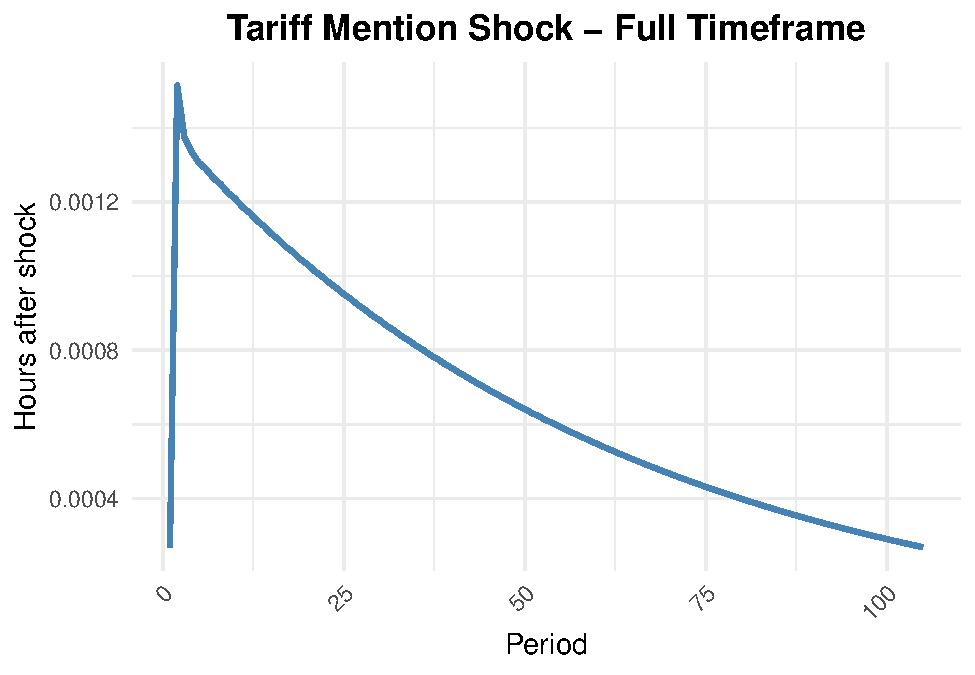
\includegraphics{_main_files/figure-latex/SPYirf-1.pdf}

\begin{Shaded}
\begin{Highlighting}[]
\CommentTok{\#irf.plot(models[["Model 4"]],nb.periods,title="Trade Mention Shock")}
\CommentTok{\#irf.plot(models[["Model 5"]],nb.periods,title="China Mention Shock")}

\FunctionTok{ggsave}\NormalTok{(}\StringTok{"armax\_plot1.png"}\NormalTok{,}\AttributeTok{plot=}\NormalTok{plot1,}\AttributeTok{bg=}\StringTok{"white"}\NormalTok{)}
\end{Highlighting}
\end{Shaded}

\section{SPY Residuals}\label{spy-residuals}

\begin{Shaded}
\begin{Highlighting}[]
\NormalTok{res1 }\OtherTok{=} \FunctionTok{checkresiduals}\NormalTok{(models[[}\StringTok{"Model 1"}\NormalTok{]], }\AttributeTok{plot =} \ConstantTok{FALSE}\NormalTok{)}
\NormalTok{res2 }\OtherTok{=} \FunctionTok{checkresiduals}\NormalTok{(models[[}\StringTok{"Model 2"}\NormalTok{]], }\AttributeTok{plot =} \ConstantTok{FALSE}\NormalTok{)}
\NormalTok{res3 }\OtherTok{=} \FunctionTok{checkresiduals}\NormalTok{(models[[}\StringTok{"Model 3"}\NormalTok{]], }\AttributeTok{plot =} \ConstantTok{FALSE}\NormalTok{)}
\NormalTok{res4 }\OtherTok{=} \FunctionTok{checkresiduals}\NormalTok{(models[[}\StringTok{"Model 4"}\NormalTok{]], }\AttributeTok{plot =} \ConstantTok{FALSE}\NormalTok{)}
\NormalTok{res5 }\OtherTok{=} \FunctionTok{checkresiduals}\NormalTok{(models[[}\StringTok{"Model 5"}\NormalTok{]], }\AttributeTok{plot =} \ConstantTok{FALSE}\NormalTok{)}
\end{Highlighting}
\end{Shaded}

\begin{Shaded}
\begin{Highlighting}[]
\NormalTok{resnames }\OtherTok{=} \FunctionTok{c}\NormalTok{(}\StringTok{"Twitter Dummy"}\NormalTok{, }\StringTok{"Twitter Count"}\NormalTok{, }\StringTok{"Tariff"}\NormalTok{, }\StringTok{"Trade"}\NormalTok{, }\StringTok{"China"}\NormalTok{)}

\CommentTok{\#extract p{-}values directly from checkresiduals results}
\NormalTok{pvals }\OtherTok{\textless{}{-}} \FunctionTok{data.frame}\NormalTok{(}\AttributeTok{Model =}\NormalTok{ resnames,}
                    \StringTok{\textasciigrave{}}\AttributeTok{Ljung{-}Box p{-}value}\StringTok{\textasciigrave{}} \OtherTok{=} \FunctionTok{c}\NormalTok{(}
\NormalTok{                      res1}\SpecialCharTok{$}\NormalTok{p.value,}
\NormalTok{                      res2}\SpecialCharTok{$}\NormalTok{p.value,}
\NormalTok{                      res3}\SpecialCharTok{$}\NormalTok{p.value,}
\NormalTok{                      res4}\SpecialCharTok{$}\NormalTok{p.value,}
\NormalTok{                      res5}\SpecialCharTok{$}\NormalTok{p.value))}

\CommentTok{\#table}
\NormalTok{knitr}\SpecialCharTok{::}\FunctionTok{kable}\NormalTok{(pvals, }\AttributeTok{digits =} \DecValTok{100}\NormalTok{, }\AttributeTok{caption =} \StringTok{"Full Timeframe Ljung{-}Box Test p{-}values"}\NormalTok{)}
\end{Highlighting}
\end{Shaded}

\begin{table}

\caption{(\#tab:SPYresiduals table)Full Timeframe Ljung-Box Test p-values}
\centering
\begin{tabular}[t]{l|r}
\hline
Model & Ljung.Box.p.value\\
\hline
Twitter Dummy & 0\\
\hline
Twitter Count & 0\\
\hline
Tariff & 0\\
\hline
Trade & 0\\
\hline
China & 0\\
\hline
\end{tabular}
\end{table}

\chapter{First Term}\label{first-term}

\begin{Shaded}
\begin{Highlighting}[]
\CommentTok{\#load final dataset}
\NormalTok{data }\OtherTok{=}\NormalTok{ backup}

\CommentTok{\#first term}
\NormalTok{data }\OtherTok{=} \FunctionTok{filter}\NormalTok{(data,}\FunctionTok{between}\NormalTok{(timestamp, }\FunctionTok{as.Date}\NormalTok{(}\StringTok{\textquotesingle{}2017{-}01{-}20\textquotesingle{}}\NormalTok{), }\FunctionTok{as.Date}\NormalTok{(}\StringTok{\textquotesingle{}2021{-}01{-}20\textquotesingle{}}\NormalTok{)))}

\CommentTok{\#for interpretation}
\NormalTok{mean2 }\OtherTok{=} \FunctionTok{mean}\NormalTok{(data}\SpecialCharTok{$}\NormalTok{SPY\_vol)}
\end{Highlighting}
\end{Shaded}

\section{SPY Models}\label{spy-models-1}

\begin{Shaded}
\begin{Highlighting}[]
\NormalTok{models }\OtherTok{\textless{}{-}} \FunctionTok{list}\NormalTok{()}

\CommentTok{\# ARMA{-}X(3,3,0) with Tariff Mentions as Exogenous}
\NormalTok{models[[}\StringTok{"First Term (1)"}\NormalTok{]] }\OtherTok{\textless{}{-}} \FunctionTok{armax}\NormalTok{(data}\SpecialCharTok{$}\NormalTok{SPY\_vol, }\AttributeTok{xreg =}\NormalTok{ data}\SpecialCharTok{$}\NormalTok{tariff, }\AttributeTok{latex =}\NormalTok{ F,}
                             \AttributeTok{nb.lags =} \DecValTok{0}\NormalTok{, }\AttributeTok{p =} \DecValTok{3}\NormalTok{, }\AttributeTok{q =} \DecValTok{3}\NormalTok{) }

\CommentTok{\# ARMA{-}X(3,3,0) with Trade Mentions as Exogenous}
\NormalTok{models[[}\StringTok{"First Term (2)"}\NormalTok{]] }\OtherTok{\textless{}{-}} \FunctionTok{armax}\NormalTok{(data}\SpecialCharTok{$}\NormalTok{SPY\_vol, }\AttributeTok{xreg =}\NormalTok{ data}\SpecialCharTok{$}\NormalTok{trade, }\AttributeTok{latex =}\NormalTok{ F,}
                             \AttributeTok{nb.lags =} \DecValTok{0}\NormalTok{, }\AttributeTok{p =} \DecValTok{3}\NormalTok{, }\AttributeTok{q =} \DecValTok{3}\NormalTok{)}

\CommentTok{\# ARMA{-}X(3,3,0) with Trade Mentions as Exogenous}
\NormalTok{models[[}\StringTok{"First Term (3)"}\NormalTok{]] }\OtherTok{\textless{}{-}} \FunctionTok{armax}\NormalTok{(data}\SpecialCharTok{$}\NormalTok{SPY\_vol, }\AttributeTok{xreg =}\NormalTok{ data}\SpecialCharTok{$}\NormalTok{china, }\AttributeTok{latex =}\NormalTok{ F,}
                             \AttributeTok{nb.lags =} \DecValTok{0}\NormalTok{, }\AttributeTok{p =} \DecValTok{3}\NormalTok{, }\AttributeTok{q =} \DecValTok{3}\NormalTok{) }
\end{Highlighting}
\end{Shaded}

\section{SPY Residuals}\label{spy-residuals-1}

\begin{Shaded}
\begin{Highlighting}[]
\NormalTok{res6 }\OtherTok{=} \FunctionTok{checkresiduals}\NormalTok{(models[[}\StringTok{"First Term (1)"}\NormalTok{]], }\AttributeTok{plot =} \ConstantTok{FALSE}\NormalTok{)}
\NormalTok{res7 }\OtherTok{=} \FunctionTok{checkresiduals}\NormalTok{(models[[}\StringTok{"First Term (2)"}\NormalTok{]], }\AttributeTok{plot =} \ConstantTok{FALSE}\NormalTok{)}
\NormalTok{res8 }\OtherTok{=} \FunctionTok{checkresiduals}\NormalTok{(models[[}\StringTok{"First Term (3)"}\NormalTok{]], }\AttributeTok{plot =} \ConstantTok{FALSE}\NormalTok{)}

\NormalTok{pvals\_new1 }\OtherTok{\textless{}{-}} \FunctionTok{data.frame}\NormalTok{(}
  \AttributeTok{Model =} \FunctionTok{c}\NormalTok{(}\StringTok{"First Term Tariffs"}\NormalTok{, }\StringTok{"First Term Trade"}\NormalTok{, }\StringTok{"First Term China"}\NormalTok{),}
  \StringTok{\textasciigrave{}}\AttributeTok{Ljung{-}Box p{-}value}\StringTok{\textasciigrave{}} \OtherTok{=} \FunctionTok{c}\NormalTok{(}
\NormalTok{    res6}\SpecialCharTok{$}\NormalTok{p.value,}
\NormalTok{    res7}\SpecialCharTok{$}\NormalTok{p.value,}
\NormalTok{    res8}\SpecialCharTok{$}\NormalTok{p.value))}
\end{Highlighting}
\end{Shaded}

\chapter{Second Term}\label{second-term}

\begin{Shaded}
\begin{Highlighting}[]
\CommentTok{\#load final dataset}
\NormalTok{data }\OtherTok{=}\NormalTok{ backup}

\CommentTok{\#second term}
\NormalTok{data }\OtherTok{=} \FunctionTok{filter}\NormalTok{(data,}\FunctionTok{between}\NormalTok{(timestamp, }\FunctionTok{as.Date}\NormalTok{(}\StringTok{\textquotesingle{}2025{-}01{-}20\textquotesingle{}}\NormalTok{), }\FunctionTok{as.Date}\NormalTok{(}\StringTok{\textquotesingle{}2025{-}05{-}07\textquotesingle{}}\NormalTok{)))}

\CommentTok{\#for interpretation}
\NormalTok{mean3 }\OtherTok{=} \FunctionTok{mean}\NormalTok{(data}\SpecialCharTok{$}\NormalTok{SPY\_vol)}
\end{Highlighting}
\end{Shaded}

\section{SPY Models}\label{spy-models-2}

\begin{Shaded}
\begin{Highlighting}[]
\CommentTok{\# ARMA{-}X(3,2,3) with Tariff Mentions as Exogenous}
\NormalTok{models[[}\StringTok{"Second Term (1)"}\NormalTok{]] }\OtherTok{\textless{}{-}} \FunctionTok{armax}\NormalTok{(data}\SpecialCharTok{$}\NormalTok{SPY\_vol, }\AttributeTok{xreg =}\NormalTok{ data}\SpecialCharTok{$}\NormalTok{tariff, }\AttributeTok{latex =}\NormalTok{ F,}
                             \AttributeTok{nb.lags =} \DecValTok{2}\NormalTok{, }\AttributeTok{p =} \DecValTok{1}\NormalTok{, }\AttributeTok{q =} \DecValTok{2}\NormalTok{) }

\CommentTok{\# ARMA{-}X(3,2,1) with Trade Mentions as Exogenous}
\NormalTok{models[[}\StringTok{"Second Term (2)"}\NormalTok{]] }\OtherTok{\textless{}{-}} \FunctionTok{armax}\NormalTok{(data}\SpecialCharTok{$}\NormalTok{SPY\_vol, }\AttributeTok{xreg =}\NormalTok{ data}\SpecialCharTok{$}\NormalTok{trade, }\AttributeTok{latex =}\NormalTok{ F,}
                             \AttributeTok{nb.lags =} \DecValTok{0}\NormalTok{, }\AttributeTok{p =} \DecValTok{1}\NormalTok{, }\AttributeTok{q =} \DecValTok{2}\NormalTok{) }

\CommentTok{\# ARMA{-}X(3,2,0) with China Mentions as Exogenous}
\NormalTok{models[[}\StringTok{"Second Term (3)"}\NormalTok{]] }\OtherTok{\textless{}{-}} \FunctionTok{armax}\NormalTok{(data}\SpecialCharTok{$}\NormalTok{SPY\_vol, }\AttributeTok{xreg =}\NormalTok{ data}\SpecialCharTok{$}\NormalTok{china, }\AttributeTok{latex =}\NormalTok{ F,}
                             \AttributeTok{nb.lags =} \DecValTok{2}\NormalTok{, }\AttributeTok{p =} \DecValTok{1}\NormalTok{, }\AttributeTok{q =} \DecValTok{2}\NormalTok{) }
\end{Highlighting}
\end{Shaded}

\section{SPY IRFs}\label{spy-irfs-1}

\begin{Shaded}
\begin{Highlighting}[]
\CommentTok{\#we want to plot the IRFs of these models}
\NormalTok{nb.periods }\OtherTok{=} \DecValTok{7} \SpecialCharTok{*} \DecValTok{15}

\NormalTok{plot2 }\OtherTok{=} \FunctionTok{irf.plot}\NormalTok{(models[[}\StringTok{"Second Term (1)"}\NormalTok{]],nb.periods,}
                 \AttributeTok{title=}\StringTok{"Tariff Mention Shock {-} Second Term"}\NormalTok{)}
\NormalTok{plot2}
\end{Highlighting}
\end{Shaded}

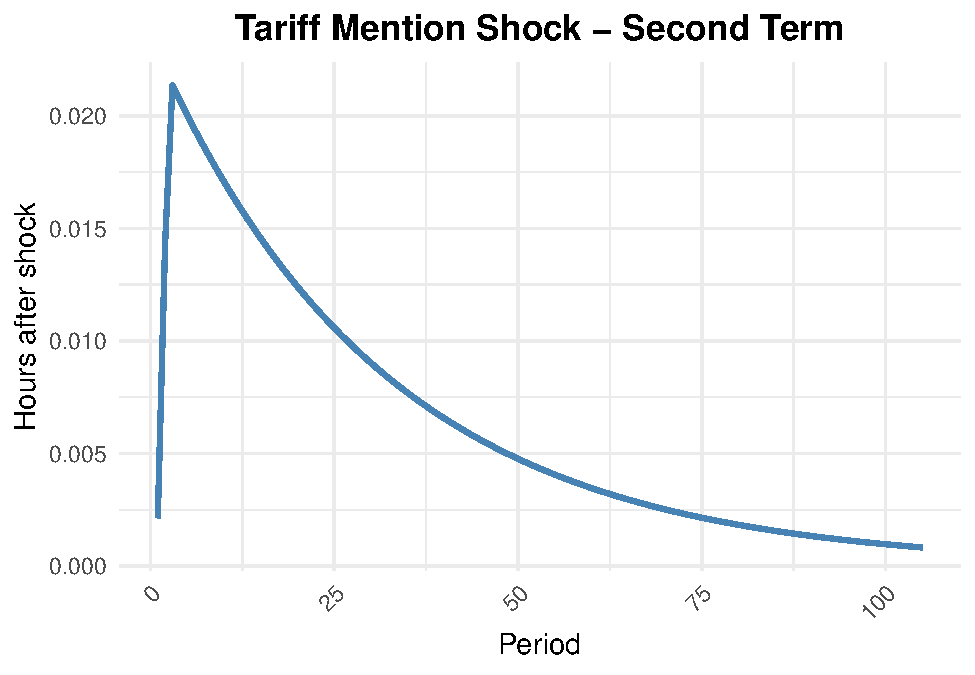
\includegraphics{_main_files/figure-latex/2nd SPYirf-1.pdf}

\begin{Shaded}
\begin{Highlighting}[]
\FunctionTok{ggsave}\NormalTok{(}\StringTok{"armax\_plot2.png"}\NormalTok{,}\AttributeTok{plot=}\NormalTok{plot2,}\AttributeTok{bg=}\StringTok{"white"}\NormalTok{)}

\NormalTok{plot3 }\OtherTok{=} \FunctionTok{irf.plot}\NormalTok{(models[[}\StringTok{"Second Term (3)"}\NormalTok{]],nb.periods,}
                 \AttributeTok{title=}\StringTok{"China Mention Shock {-} Second Term"}\NormalTok{)}
\NormalTok{plot3}
\end{Highlighting}
\end{Shaded}

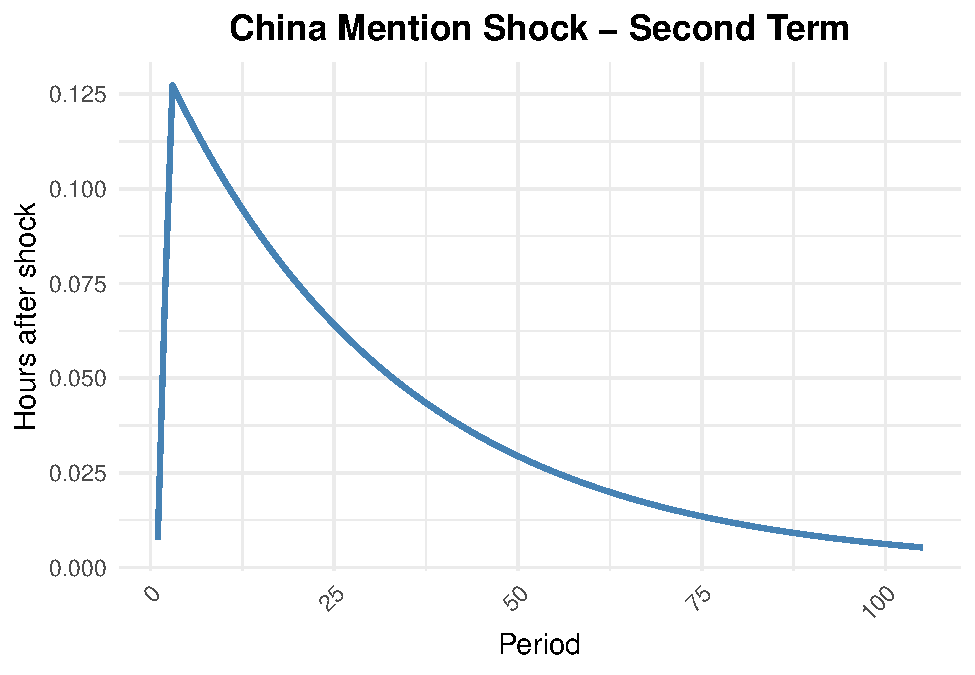
\includegraphics{_main_files/figure-latex/2nd SPYirf-2.pdf}

\section{SPY Residuals}\label{spy-residuals-2}

\begin{Shaded}
\begin{Highlighting}[]
\NormalTok{res9 }\OtherTok{=} \FunctionTok{checkresiduals}\NormalTok{(models[[}\StringTok{"Second Term (1)"}\NormalTok{]], }\AttributeTok{plot =} \ConstantTok{FALSE}\NormalTok{)}
\NormalTok{res10 }\OtherTok{=} \FunctionTok{checkresiduals}\NormalTok{(models[[}\StringTok{"Second Term (2)"}\NormalTok{]], }\AttributeTok{plot =} \ConstantTok{FALSE}\NormalTok{)}
\NormalTok{res11 }\OtherTok{=} \FunctionTok{checkresiduals}\NormalTok{(models[[}\StringTok{"Second Term (3)"}\NormalTok{]], }\AttributeTok{plot =} \ConstantTok{FALSE}\NormalTok{)}

\NormalTok{pvals\_new2 }\OtherTok{\textless{}{-}} \FunctionTok{data.frame}\NormalTok{(}
  \AttributeTok{Model =} \FunctionTok{c}\NormalTok{(}\StringTok{"Second Term Tariffs"}\NormalTok{, }\StringTok{"Second Term Trade"}\NormalTok{, }\StringTok{"Second Term China"}\NormalTok{),}
  \StringTok{\textasciigrave{}}\AttributeTok{Ljung{-}Box p{-}value}\StringTok{\textasciigrave{}} \OtherTok{=} \FunctionTok{c}\NormalTok{(}
\NormalTok{    res9}\SpecialCharTok{$}\NormalTok{p.value,}
\NormalTok{    res10}\SpecialCharTok{$}\NormalTok{p.value,}
\NormalTok{    res11}\SpecialCharTok{$}\NormalTok{p.value))}

\CommentTok{\#combine with other term}
\NormalTok{pvals\_combined }\OtherTok{\textless{}{-}} \FunctionTok{rbind}\NormalTok{(pvals\_new1, pvals\_new2)}
\end{Highlighting}
\end{Shaded}

\section{SPY Table (both terms)}\label{spy-table-both-terms}

\centering

Table: \label{tab:armax1} Split-Term ARMAX Models of Average Hourly Volatility

\begin{Shaded}
\begin{Highlighting}[]
\FunctionTok{library}\NormalTok{(modelsummary)}

\NormalTok{xnames }\OtherTok{\textless{}{-}} \FunctionTok{c}\NormalTok{(}
  \StringTok{"ar1"} \OtherTok{=} \StringTok{"AR(1)"}\NormalTok{,}
  \StringTok{"ar2"} \OtherTok{=} \StringTok{"AR(2)"}\NormalTok{,}
  \StringTok{"ar3"} \OtherTok{=} \StringTok{"AR(3)"}\NormalTok{,}
  \StringTok{"ma1"} \OtherTok{=} \StringTok{"MA(1)"}\NormalTok{,}
  \StringTok{"ma2"} \OtherTok{=} \StringTok{"MA(2)"}\NormalTok{,}
  \StringTok{"ma3"} \OtherTok{=} \StringTok{"MA(3)"}\NormalTok{,}
  \StringTok{"(Intercept)"} \OtherTok{=} \StringTok{"Constant"}\NormalTok{,}
  \StringTok{"tariff\_lag\_0"} \OtherTok{=} \StringTok{"$Tariff\_\{t\}$"}\NormalTok{,}
  \StringTok{"tariff\_lag\_1"} \OtherTok{=} \StringTok{"$Tariff\_\{t{-}1\}$"}\NormalTok{,}
  \StringTok{"tariff\_lag\_2"} \OtherTok{=} \StringTok{"$Tariff\_\{t{-}2\}$"}\NormalTok{,}
  \StringTok{"trade\_lag\_0"} \OtherTok{=} \StringTok{"$Trade\_\{t\}$"}\NormalTok{,}
  \StringTok{"china\_lag\_0"} \OtherTok{=} \StringTok{"$China\_\{t\}$"}\NormalTok{,}
  \StringTok{"china\_lag\_1"} \OtherTok{=} \StringTok{"$China\_\{t{-}1\}$"}\NormalTok{,}
  \StringTok{"china\_lag\_2"} \OtherTok{=} \StringTok{"$China\_\{t{-}2\}$"}
\NormalTok{)}

\FunctionTok{msummary}\NormalTok{(models,}
         \AttributeTok{coef\_map =}\NormalTok{ xnames,}
         \AttributeTok{stars =} \FunctionTok{c}\NormalTok{(}\StringTok{\textquotesingle{}*\textquotesingle{}} \OtherTok{=} \FloatTok{0.05}\NormalTok{, }\StringTok{\textquotesingle{}**\textquotesingle{}} \OtherTok{=} \FloatTok{0.01}\NormalTok{, }\StringTok{\textquotesingle{}***\textquotesingle{}} \OtherTok{=} \FloatTok{0.001}\NormalTok{),}
         \AttributeTok{output =} \StringTok{"markdown"}\NormalTok{,   }\CommentTok{\# or "latex" for PDF, or "html" for HTML output}
         \AttributeTok{title =} \StringTok{"Split{-}Term ARMAX Models of Average Hourly Volatility"}\NormalTok{,}
         \AttributeTok{fmt =} \DecValTok{4}\NormalTok{,}
         \AttributeTok{estimate =} \StringTok{"\{estimate\}\{stars\}"}\NormalTok{,}
         \AttributeTok{gof\_omit =} \StringTok{"IC|Log|Num. obs."}
\NormalTok{)}
\end{Highlighting}
\end{Shaded}

\begin{table}
\centering
\begin{talltblr}[         %% tabularray outer open
caption={Split-Term ARMAX Models of Average Hourly Volatility},
]                     %% tabularray outer close
{                     %% tabularray inner open
colspec={Q[]Q[]Q[]Q[]Q[]Q[]Q[]},
column{2,3,4,5,6,7}={}{halign=c,},
column{1}={}{halign=l,},
hline{28}={1,2,3,4,5,6,7}{solid, black, 0.05em},
}                     %% tabularray inner close
\toprule
& First Term (1) & First Term (2) & First Term (3) & Second Term (1) & Second Term (2) & Second Term (3) \\ \midrule %% TinyTableHeader
AR(1) & 0.2953*** & 0.2943*** & 0.2927*** & 0.9686*** & 0.9683*** & 0.9693*** \\
& (0.0225) & (0.0224) & (0.0224) & (0.0163) & (0.0163) & (0.0161) \\
AR(2) & 0.1434*** & 0.1439*** & 0.1438*** &  &  &  \\
& (0.0220) & (0.0220) & (0.0219) &  &  &  \\
AR(3) & 0.5456*** & 0.5462*** & 0.5480*** &  &  &  \\
& (0.0223) & (0.0222) & (0.0222) &  &  &  \\
MA(1) & 0.1854*** & 0.1863*** & 0.1866*** & -0.6965*** & -0.6905*** & -0.7207*** \\
& (0.0180) & (0.0179) & (0.0179) & (0.0469) & (0.0469) & (0.0467) \\
MA(2) & -0.1707*** & -0.1706*** & -0.1695*** & -0.1732*** & -0.1755*** & -0.1609*** \\
& (0.0169) & (0.0169) & (0.0168) & (0.0437) & (0.0438) & (0.0434) \\
MA(3) & -0.6557*** & -0.6564*** & -0.6575*** &  &  &  \\
& (0.0162) & (0.0161) & (0.0161) &  &  &  \\
$Tariff_{t}$ & 0.0011 &  &  & 0.0048 &  &  \\
& (0.0010) &  &  & (0.0099) &  &  \\
$Tariff_{t-1}$ &  &  &  & 0.0278** &  &  \\
&  &  &  & (0.0102) &  &  \\
$Tariff_{t-2}$ &  &  &  & 0.0168 &  &  \\
&  &  &  & (0.0099) &  &  \\
$Trade_{t}$ &  & 0.0023** &  &  & -0.0074 &  \\
&  & (0.0009) &  &  & (0.0297) &  \\
$China_{t}$ &  &  & 0.0018** &  &  & 0.0173 \\
&  &  & (0.0006) &  &  & (0.0319) \\
$China_{t-1}$ &  &  &  &  &  & 0.1515*** \\
&  &  &  &  &  & (0.0324) \\
$China_{t-2}$ &  &  &  &  &  & 0.1309*** \\
&  &  &  &  &  & (0.0319) \\
Num.Obs. & 7042 & 7042 & 7042 & 516 & 518 & 516 \\
RMSE & 0.03 & 0.03 & 0.03 & 0.44 & 0.44 & 0.43 \\
\bottomrule
\end{talltblr}
\end{table}

\chapter{Descriptive Stats}\label{descriptive-stats}

\begin{Shaded}
\begin{Highlighting}[]
\NormalTok{means }\OtherTok{\textless{}{-}} \FunctionTok{data.frame}\NormalTok{(}
  \AttributeTok{Model =} \FunctionTok{c}\NormalTok{(}\StringTok{"Full Time Mean"}\NormalTok{, }\StringTok{"First Term Mean"}\NormalTok{, }\StringTok{"Second Term Mean"}\NormalTok{),}
  \StringTok{\textasciigrave{}}\AttributeTok{SPY Volatility Mean}\StringTok{\textasciigrave{}} \OtherTok{=} \FunctionTok{c}\NormalTok{(}
\NormalTok{    mean1,}
\NormalTok{    mean2,}
\NormalTok{    mean3))}

\NormalTok{table4 }\OtherTok{=}\NormalTok{ knitr}\SpecialCharTok{::}\FunctionTok{kable}\NormalTok{(means, }\AttributeTok{digits =} \DecValTok{6}\NormalTok{, }\AttributeTok{format=}\StringTok{"latex"}\NormalTok{,}
             \AttributeTok{caption =} \StringTok{"Summary Statistics of SPY Volatility"}\NormalTok{)}

\NormalTok{table4}
\end{Highlighting}
\end{Shaded}

\begin{table}

\caption{\label{tab:means}Summary Statistics of SPY Volatility}
\centering
\begin{tabular}[t]{l|r}
\hline
Model & SPY.Volatility.Mean\\
\hline
Full Time Mean & 0.022621\\
\hline
First Term Mean & 0.017486\\
\hline
Second Term Mean & 0.144248\\
\hline
\end{tabular}
\end{table}

\chapter{Cross-references}\label{cross}

Cross-references make it easier for your readers to find and link to elements in your book.

\section{Chapters and sub-chapters}\label{chapters-and-sub-chapters}

There are two steps to cross-reference any heading:

\begin{enumerate}
\def\labelenumi{\arabic{enumi}.}
\tightlist
\item
  Label the heading: \texttt{\#\ Hello\ world\ \{\#nice-label\}}.

  \begin{itemize}
  \tightlist
  \item
    Leave the label off if you like the automated heading generated based on your heading title: for example, \texttt{\#\ Hello\ world} = \texttt{\#\ Hello\ world\ \{\#hello-world\}}.
  \item
    To label an un-numbered heading, use: \texttt{\#\ Hello\ world\ \{-\#nice-label\}} or \texttt{\{\#\ Hello\ world\ .unnumbered\}}.
  \end{itemize}
\item
  Next, reference the labeled heading anywhere in the text using \texttt{\textbackslash{}@ref(nice-label)}; for example, please see Chapter \ref{cross}.

  \begin{itemize}
  \tightlist
  \item
    If you prefer text as the link instead of a numbered reference use: \hyperref[cross]{any text you want can go here}.
  \end{itemize}
\end{enumerate}

\section{Captioned figures and tables}\label{captioned-figures-and-tables}

Figures and tables \emph{with captions} can also be cross-referenced from elsewhere in your book using \texttt{\textbackslash{}@ref(fig:chunk-label)} and \texttt{\textbackslash{}@ref(tab:chunk-label)}, respectively.

See Figure \ref{fig:nice-fig}.

\begin{Shaded}
\begin{Highlighting}[]
\FunctionTok{par}\NormalTok{(}\AttributeTok{mar =} \FunctionTok{c}\NormalTok{(}\DecValTok{4}\NormalTok{, }\DecValTok{4}\NormalTok{, .}\DecValTok{1}\NormalTok{, .}\DecValTok{1}\NormalTok{))}
\FunctionTok{plot}\NormalTok{(pressure, }\AttributeTok{type =} \StringTok{\textquotesingle{}b\textquotesingle{}}\NormalTok{, }\AttributeTok{pch =} \DecValTok{19}\NormalTok{)}
\end{Highlighting}
\end{Shaded}

\begin{figure}

{\centering 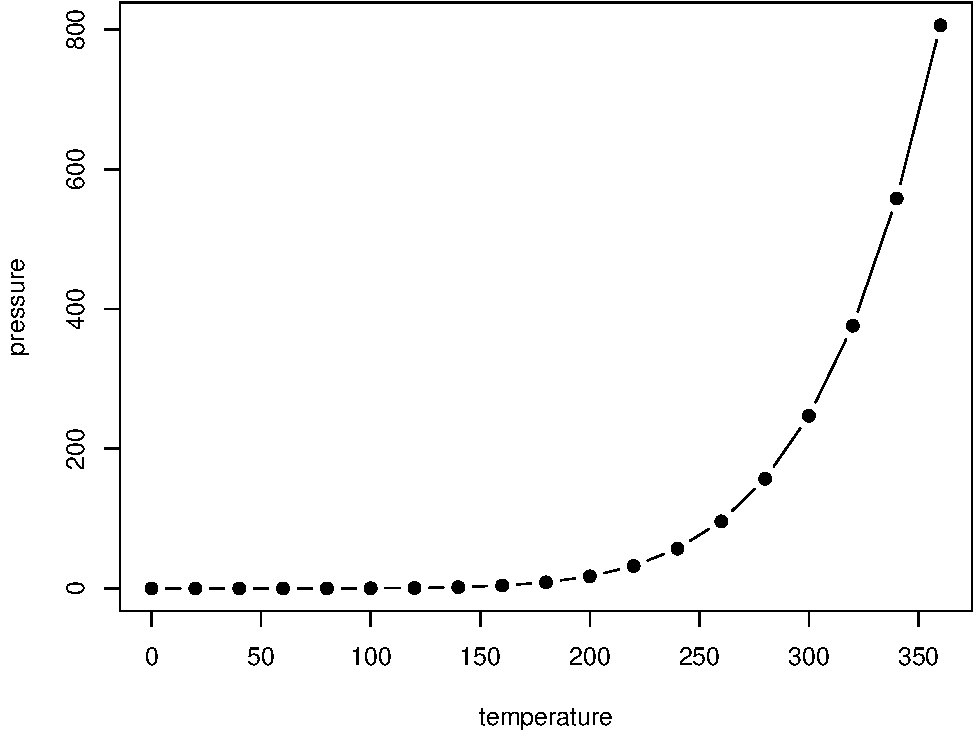
\includegraphics[width=0.8\linewidth,alt={Plot with connected points showing that vapor pressure of mercury increases exponentially as temperature increases.}]{_main_files/figure-latex/nice-fig-1} 

}

\caption{Here is a nice figure!}\label{fig:nice-fig}
\end{figure}

Don't miss Table \ref{tab:nice-tab}.

\begin{Shaded}
\begin{Highlighting}[]
\NormalTok{knitr}\SpecialCharTok{::}\FunctionTok{kable}\NormalTok{(}
  \FunctionTok{head}\NormalTok{(pressure, }\DecValTok{10}\NormalTok{), }\AttributeTok{caption =} \StringTok{\textquotesingle{}Here is a nice table!\textquotesingle{}}\NormalTok{,}
  \AttributeTok{booktabs =} \ConstantTok{TRUE}
\NormalTok{)}
\end{Highlighting}
\end{Shaded}

\begin{table}

\caption{\label{tab:nice-tab}Here is a nice table!}
\centering
\begin{tabular}[t]{rr}
\toprule
temperature & pressure\\
\midrule
0 & 0.0002\\
20 & 0.0012\\
40 & 0.0060\\
60 & 0.0300\\
80 & 0.0900\\
\addlinespace
100 & 0.2700\\
120 & 0.7500\\
140 & 1.8500\\
160 & 4.2000\\
180 & 8.8000\\
\bottomrule
\end{tabular}
\end{table}

  \bibliography{macroeconometrics\_citations.bib}

\end{document}
